\documentclass[11pt]{article}
\usepackage[a4paper,margin=22mm]{geometry}
\usepackage[T1]{fontenc}
\usepackage{lmodern,microtype,amsmath,amssymb,booktabs,tabularx,longtable,graphicx,hyperref,placeins}
\emergencystretch=2em
\title{Supplementary information\\Few-label calibration under publication shift in catalysis}
\author{}\date{}
\usepackage{pdflscape}
\begin{document}\maketitle
\section{Analysis populations and provenance}
Historical cleaned input snapshots are inherited from the supplied research archive; the preceding full-study release refit the controlled split analysis and established a traceable source-tuned adaptation engine. It does not claim independent re-extraction of every historical measurement or restoration of the original archive's missing executed-engine version. Rows preserve original-file and row identifiers; historical OCM includes the row-audit table. The cleaned snapshots, their hashes and actual train/test ledgers are the reproducible starting point. Historical raw-file curation exclusions are not represented as newly independently audited extraction decisions.

The methanol paired corpus has 1,245 rows, 82 sources and 80 leakage groups; STY has 1,230 rows and 109 sources; OCM has 1,794 rows, 408 sources and 405 groups. Methanol and STY share 20 publication identifiers. OCM F0/F1 have identical outcome and source populations. All reported targets are finite; genuine zeros remain observations. Required operating-variable meanings follow the released upstream datasets. Missing operating values are imputed using a median fitted on the current training rows; an entirely missing training column uses the documented keep-empty-feature behavior. Numeric scaling also uses only that partition. No target-source query feature values extend composition vocabularies.
\small\begin{longtable}{llrrr}
\caption{Historical input quality, recomputed from distributed snapshots.}\\
\toprule Panel & Feature & Missing & Minimum & Maximum \\ \midrule\endfirsthead
\toprule Panel & Feature & Missing & Minimum & Maximum \\ \midrule\endhead
\bottomrule\endfoot
methanol & Temperature\_K & 0 & 433 & 673 \\
methanol & Pressure\_bar & 0 & 0.4 & 80 \\
methanol & H2\_CO2\_ratio & 0 & 1 & 10 \\
methanol & GHSV\_L\_g\_h & 77 & 0.87 & 240 \\
methanol & BET\_surface\_area\_m2\_g & 230 & 2 & 974.9 \\
ocm\_f0 & Temperature\_K & 0 & 773 & 1223 \\
ocm\_f0 & CH4\_partial\_pressure\_bar & 0 & 0.0094 & 2.7 \\
ocm\_f0 & O2\_partial\_pressure\_bar & 0 & 0.003 & 1.35 \\
ocm\_f0 & CH4\_O2\_ratio & 0 & 0.8 & 38.31 \\
ocm\_f0 & total\_pressure\_bar & 0 & 0.106 & 4.5 \\
ocm\_f0 & contact\_time\_s & 44 & 0.0017 & 182.5 \\
sty & Temperature\_K & 0 & 433 & 673 \\
sty & Pressure\_bar & 0 & 1 & 360 \\
sty & H2\_CO2\_ratio & 0 & 1 & 20 \\
sty & GHSV\_L\_g\_h & 0 & 0.9 & 120 \\
sty & SBET\_m2\_g & 0 & 2 & 1102 \\
\end{longtable}\normalsize
There are 497 missing catalyst names in the paired methanol data. The name holdout uses only nonempty normalized strings and requires a complete eligible stratum; it does not identify a physical preparation batch. The STY operating snapshot has no catalyst-name field. Richer public Suvarna metadata are retained in the retrieved workbook but are not retroactively added to this operating-input benchmark. The OCM catalyst number identifies an upstream record, not repeated measurements certified on one physical catalyst.

\section{Chronology and claim scope}
The historical adaptation study is retrospective: archived outcomes motivated its research question. The new-source protocol was locally timestamped and hashed before new query outcomes were evaluated, not independently preregistered. Its primary hypothesis is the five-label composition-enriched blend versus local response contrast. Bibliographic identity corrections remove re-listed old sources even when spelling or number changes; no error-dependent inclusion is used. The additional compilation is a separately released source of observations, rather than a prospective laboratory campaign.

The label-permutation, matched-alpha and fit-regime sensitivity analyses are explanatory follow-ups, not replacements for the frozen primary test. The latter uses every one of the 25 historical outer-training fits; no fit is selected by external performance. Fixed ridge/boosting split audits on old data are retrospective, with configuration held constant within each comparison. Published-workflow audits serve a separate question about validation scope. Suvarna numbers are recomputed from archived predictions; Xu's matched five-fold grouping comparison is newly refitted with XGBoost 3.2.0. Neither is external validation of the new adapters.

\section{Split and support construction}
Historical outer folds are stored in leakage-group split ledgers, with seeds 42, 101, 202, 303 and 404. Each seed covers every row exactly once as an outer test observation. Training inner folds randomly permute sorted leakage-group identities into three blocks. All imputation/scaling/composition encoders are fitted on the relevant inner training block before OOF prediction.

For a source with $n$ records, sort row identifiers, shuffle with a stable SHA-derived identifier seed, and query $\max(5,\lceil n/4\rceil)$ rows. Remaining rows are the support pool. A complete curve requires ten pool records. Fifty independently seeded pool orders create nested budgets 1, 2, 3, 5 and 10; the same order is used for every method. No support record is also a query. Calibration labels are disclosed to the prediction function only for that budget.

High-temperature design enumerates observed cutoffs and selects the upper block closest to a quarter of available finite-temperature records, subject to at least five queries and ten strictly lower-temperature pool rows. It never splits tied temperatures across support and query. Name-stratum design enumerates complete reported-name strata with the same minimum sizes and selects the query size closest to a quarter; it never places the same normalized name on both sides. Stress hyperparameters are frozen from random-source training. Matched-source random panels are available for interpretation, but their query records differ from stress panels, so these contrasts are not causal measurements of a difficulty increase.

\section{All nine strategies}
Let $p_A=f_G(A)$, $p_T=f_G(T)$, support responses $y_A$, support residual mean $\bar r$, and historical response scale $s>0$.
\begin{enumerate}
\item Global: $q=p_T$, a zero-support-label reference at every plotted budget.
\item Support mean: $q=\bar y_A$.
\item Offset: $q=p_T+\bar r$.
\item Affine: $z_A=(p_A-\bar p_A)/s$, $z_T=(p_T-\bar p_A)/s$,
\[q=p_T+\bar r+z_T\frac{z_A^\top(y_A-p_A)}{z_A^\top z_A+\lambda}.\]
This shrinks the additional slope toward an offset map, with an unpenalized residual mean.
\item Empirical-Bayes offset: $q=p_T+\mu+\eta_k(\bar r-\mu)$,
\[\eta_k=\frac{k\tau^2}{\sigma^2+k\tau^2}.\]
Historical OOF residuals provide the source-equal residual mean $\mu$, pooled within-source variance $\sigma^2$, and between-source variance corrected for within-source mean noise, truncated below at zero. The variance floor is $10^{-12}$.
\item Local ridge: fit $y_A$ on training-fitted $z_A$, intercept unpenalized.
\item Temperature ridge: the same support fit using only the scaled temperature coordinate.
\item Residual ridge: fit $y_A-p_A$ on $z_A$ and add $p_T$.
\item Shrinkage blend: combine local and residual predictions with support leave-one-out and historical pseudo-source shrinkage, as specified in the main text.
\end{enumerate}
Ridge/affine strengths are separately selected per method and label budget from $\{.1,1,10,100\}$. Ties follow the declared grid order. The base grid has four ridge candidates; boosting candidates (100,2), (100,3), (300,2), (300,3), (500,8), where pairs are trees/depth. Boosting uses learning rate .05, subsample .8, minimum split size 3 and random state 42. Its candidate score is source-equal absolute OOF error, not pooled record MAE.

Adapters are scored on ten training-source pseudo-support draws per budget. Local, residual, temperature and affine strengths minimize source-equal pseudo-query MAE. For blending, prior $w_0\in\{0,.25,.5,.75,1\}$ minimizes pseudo-query error; disagreement scale is the source-equal mean component leave-one-out squared difference (one-label query disagreement at $k=1$). Shrinkage $c\in\{\infty,10,2,.5,0\}$ is selected with the prior/scale for each pseudo-source excluding its leakage group. Actual outer or additional-source query labels are not used. Reuse of training pseudo-queries across hyperparameter stages can affect training selection, but final outer and additional-source assessments remain separate.

\section{Exact ridge leave-one-out and projection identity}
Center support matrix $X$ and responses $y$ without penalizing the intercept. For $k$ support records, let $K=X_cX_c^\top$, $B=(K+\alpha I)^{-1}$, and
\[\widehat y_T=\bar y+(X_T-\bar X)X_c^\top B(y-\bar y).\]
The diagonal leverage is $h_i=1/k+(KB)_{ii}$. For $k>1$ the exact leave-one-out response prediction is
\[\widehat y_{-i}=y_i-\frac{y_i-\widehat y_i}{1-h_i}.\]
This uses fixed historical transformations; it does not refit the historical preprocessing on support labels. Independent mathematical verification compares predictions with scikit-learn Ridge and leave-one-out refits.

For fixed features, the map from $y_A$ to query predictions is linear. Therefore
\[R_\alpha[y_A-p_A]=R_\alpha[y_A]-R_\alpha[p_A],\quad q_R-q_L=p_T-R_\alpha[p_A].\]
The main method chooses its two alphas separately. In the exploratory matched-alpha ablation, both use the selected local alpha without new tuning. The identity is checked numerically for all historical OCM and additional-source random draws at $k=5$. An added global component can correct a local response or add error; linearity alone does not determine which.

\section{Additional OCM source reconstruction}
The public updated workbook has 4,759 rows and 533 represented publication numbers. The old bibliography has 420 unique numbers up to 421, including an ambiguous duplicated number. Existing numbers are conservatively old, even when their citation text has a typographic change. Additional numbers are screened against normalized old citations and bibliometric fields. Three aliases are removed: 424=396, 427=395 and 429=105, leaving 118 additional bibliographic entries before record-quality eligibility. Four old-number citation differences are logged; two concern missing old citation strings and the others typography. They do not qualify as new sources.

Admitted new records require finite positive temperature, partial pressures, pressure ratio and total pressure; contact time may be missing but cannot be nonpositive when observed. C$_2$ yield must be reported within $[0,100]$. Composition encoding validates species/amount pairing and amount range; a fifth/sixth cation or third support cannot be omitted to fit the frozen schema. Full upstream record duplicates are removed. The exclusion reasons overlap: 1,845 records are old/unverifiable publications, 393 lack valid CH$_4$ partial pressure, 393 lack valid O$_2$ partial pressure, 100 exceed slots, 44 lack a valid target, and 21 are full duplicates. Their sum is not the excluded-row count. Exactly 2,378 distinct rows are excluded, leaving 2,381 from 91 sources.

The workbook describes species amounts as molar percentages, pressures in bar, temperature in K, contact time in s and C$_2$ yield as methane conversion times combined C$_2$ selectivity. We preserve these reported variables rather than infer pressure assumptions or physical absence from blank slots. The complete row-audit, all-source registry and bibliography screen are distributed. The 52-source main cohort and 40-source high-temperature cohort have label-blind design ledgers and shared F0/F1 support orders.

The full-fit F1 backbone is gradient boosting (500,8). At $k=5$, local and residual alphas are both 1, affine strength 1, temperature alpha 1, blend prior .5, shrinkage 10 and disagreement scale 6.6618. F0 backbone is (100,3); local alpha 10, residual alpha 100, affine .1, temperature 1, blend prior 0, shrinkage 10 and scale 1.4613. These settings come exclusively from old OCM sources. Serialized backbones, preprocessing parameters, training OOF records and all selection scores are saved.
\small\begin{longtable}{r p{.39\linewidth} rrrr}
\caption{Additional OCM main-cohort sources. No. is the public update bibliography number; n is the number of admitted records. Errors are pp at k=5.}\\
\toprule No. & Citation & n & Local & Blend & $\Delta$ \\ \midrule\endfirsthead
\toprule No. & Citation & n & Local & Blend & $\Delta$ \\ \midrule\endhead
\bottomrule\endfoot
422 & Appl. Catal. A Gen. 219 (2001) 61-68 & 37 & 2.927 & 3.041 & 0.114 \\
423 & Appl. Catal. A Gen. 354 (2009) 143--152 & 60 & 0.570 & 0.753 & 0.183 \\
425 & Ind. Eng. Chem. Res. 48 (2009) 641--646 & 65 & 1.853 & 1.670 & -0.183 \\
431 & J. Nat. Gas Chem. 19 (2010) 35--42 & 20 & 3.420 & 2.489 & -0.931 \\
434 & J. Nat. Gas Chem. 19 (2010) 534--538 & 20 & 3.302 & 2.041 & -1.260 \\
435 & J. Nat. Gas Chem. 19 (2010) 25--30 & 30 & 1.773 & 1.821 & 0.048 \\
439 & Appl. Catal. A Gen. 375 (2010) 172--178 & 52 & 2.133 & 2.102 & -0.031 \\
444 & J. Nat. Gas Chem. 20 (2011) 204--213 & 45 & 7.283 & 7.467 & 0.184 \\
445 & J. Nat. Gas Chem. 20 (2011) 428--434 & 63 & 4.575 & 3.853 & -0.722 \\
446 & J. Mol. Catal. A Chem. 346 (2011) 46--54 & 52 & 2.196 & 2.330 & 0.134 \\
447 & Appl. Catal. A Gen. 406 (2011) 1--12 & 54 & 4.498 & 4.643 & 0.145 \\
448 & Appl. Catal. A Gen. 391 (2011) 205--214 & 28 & 3.285 & 3.223 & -0.063 \\
449 & J. Catal. 281 (2011) 241--253 & 19 & 4.873 & 4.756 & -0.118 \\
451 & J. Nat. Gas Chem. 21 (2012) 49--55 & 27 & 9.719 & 8.658 & -1.061 \\
455 & Asian Journal of Chemistry 25 (2013) 9179-9184 & 35 & 3.009 & 3.189 & 0.180 \\
457 & Appl. Catal. A Gen. 454 (2013) 100--114 & 50 & 1.466 & 1.250 & -0.217 \\
466 & Appl. Catal. A Gen. 485 (2014) 10--19  & 36 & 4.163 & 4.506 & 0.343 \\
467 & ACS Catal. 4 (2014) 1972--1990 & 62 & 4.062 & 4.185 & 0.122 \\
468 & Appl. Catal. A Gen. 484 (2014) 97--107 & 25 & 4.732 & 4.446 & -0.286 \\
469 & Inorg. Mater. 50 (2014) 912--916 & 17 & 3.849 & 4.261 & 0.413 \\
470 & Appl. Catal. A Gen. 472 (2014) 39--46 & 23 & 5.613 & 5.432 & -0.182 \\
471 & Dokl. Phys. Chem. 455 (2014) 60--63 & 18 & 3.294 & 3.592 & 0.298 \\
472 & Catal. Today 228 (2014) 5--14 & 67 & 1.760 & 2.292 & 0.532 \\
476 & React. Kinet. Mech. Catal. 112 (2014) 227--240 & 21 & 4.086 & 4.135 & 0.049 \\
480 & Appl. Catal. B Environ. 150--151 (2014) 496--505 & 21 & 9.759 & 9.728 & -0.031 \\
481 & Nanoscale 7 (2015) 2260--2264 & 87 & 5.825 & 5.945 & 0.120 \\
482 & J. Catal. 329, (2015), 560--573 & 26 & 0.432 & 0.479 & 0.048 \\
485 & ACS Catal. 5 (2015) 1663--1674 & 20 & 7.073 & 7.024 & -0.049 \\
486 & Pet. Chem. 55 (2015) 163--168  & 39 & 3.438 & 3.481 & 0.043 \\
492 & Appl. Catal. A Gen. 528 (2016) 175--190 & 140 & 3.912 & 3.910 & -0.002 \\
496 & RSC Adv. 6 (2016) 34872--34876 & 32 & 1.246 & 1.296 & 0.050 \\
503 & Appl. Catal. A Gen. 537 (2017) 33--39  & 57 & 1.883 & 1.971 & 0.088 \\
504 & Sci. Adv. 3, (2017) & 47 & 3.181 & 3.022 & -0.159 \\
506 & Appl. Catal. A Gen. 544 (2017) 77--83 & 48 & 2.532 & 2.556 & 0.024 \\
508 & Mol. Catal. 435 (2017) 13--23 & 19 & 2.221 & 2.316 & 0.095 \\
510 & ACS Comb. Sci. 19 (2017) 15--24  & 32 & 1.262 & 1.396 & 0.135 \\
514 & ChemNanoMat 4 (2018) 487--495 & 44 & 5.470 & 5.647 & 0.177 \\
515 & Appl. Catal. A Gen. 552 (2018) 117--128 & 31 & 6.306 & 5.840 & -0.466 \\
516 & Catal. Today 299 (2018) 60--66  & 23 & 4.515 & 4.592 & 0.078 \\
520 & Chinese J. Catal. 39 (2018) 1395--1402 & 30 & 5.390 & 5.383 & -0.007 \\
521 & Front. Chem. 6 (2018) 1--10 & 36 & 2.325 & 2.354 & 0.029 \\
522 & Eur. J. Inorg. Chem. (2018) 1787--1799 & 40 & 1.853 & 1.924 & 0.071 \\
523 & Chem. Eng. Sci. 175 (2018) 199--207 & 22 & 2.275 & 2.421 & 0.146 \\
526 & Mol. Catal. 457 (2018) 74--81  & 27 & 1.930 & 2.000 & 0.070 \\
527 & Inorg. Chem. Commun. 100 (2019) 97--100 & 28 & 5.725 & 5.490 & -0.235 \\
528 & ACS Catal. 9 (2019) 4030--4045 & 18 & 3.406 & 3.711 & 0.305 \\
529 & Mol. Catal. 470 (2019) 40--47 & 146 & 1.595 & 1.796 & 0.201 \\
531 & J. Catal. 375 (2019) 478--492 & 26 & 4.362 & 4.578 & 0.217 \\
535 & Eur. J. Inorg. Chem. 2 (2019) 183--194 & 30 & 3.588 & 3.385 & -0.203 \\
536 & Polyhedron 170 (2019) 602--611 & 63 & 1.200 & 1.175 & -0.024 \\
537 & Chinese Chem. Lett. 30 (2019) 1141--1146 & 25 & 2.919 & 2.318 & -0.601 \\
539 & Ind. Eng. Chem. Res. 58 (2019) 22847--22856 & 24 & 2.746 & 2.803 & 0.057 \\
\end{longtable}\normalsize

\section{Metric estimands and uncertainty}
Let $e_{srj}$ be query MAE for source $s$, support repeat $r$ and historical outer seed $j$. Historical source MAE is $\bar e_s=\frac1J\sum_j\frac1R\sum_r e_{srj}$, and the primary benchmark MAE is $\frac1S\sum_s\bar e_s$. External full-fit MAE omits the seed average. Row-weighted sensitivity weights each source by its fixed query count. Bounded sensitivity clips percentage predictions to $[0,100]$ and STY predictions below at zero; raw observations are unchanged.

Cluster bootstrap samples leakage groups with replacement and divides sampled source-error sums by sampled source counts. It does not replace the source-equal estimand with group-equal averaging. Twenty thousand draws estimate percentile intervals, conditional on the fitted models and observed sources. No adjustment across secondary comparisons is applied. A zero-crossing interval is neither equivalence nor proof of no effect. Identical within-source control outputs can yield numerical differences near floating-point precision.

Stacked repeated $R^2$ is $1-\sum_{sjri}(y_i-p_i)^2/\sum_{sjri}(y_i-\bar y)^2$ over the specified repeated prediction population. $R^2$ of a mean prediction instead averages each record's predictions before squaring the error; these are different quantities. The main controlled audit uses the former. An older archive field named prediction-averaged $R^2$ actually averaged squared errors before forming $R^2$; that label is not retained as an averaged-prediction metric.

\section{Complete budget tables}
Values below are source-equal raw MAEs. Units are pp for percent targets and mg MeOH h$^{-1}$ g$_{cat}^{-1}$ for STY. Stress cohorts and selected parameters are fixed across budgets. Intervals, bounded/row-weighted sensitivities and paired source values accompany the CSV exports; printed tables avoid pretending that support repeats increase the number of independent sources.
\subsubsection*{Historical / methanol / CO2\_conversion\_percent / random}
\begin{center}\small
\begin{tabular}{lrrrrr}
\toprule
Strategy & k=1 & k=2 & k=3 & k=5 & k=10 \\
\midrule
Global & 5.271 & 5.271 & 5.271 & 5.271 & 5.271 \\
Support mean & 5.309 & 4.616 & 4.420 & 4.304 & 4.146 \\
Offset & 4.269 & 3.727 & 3.556 & 3.455 & 3.329 \\
Affine & 4.269 & 3.635 & 3.336 & 3.083 & 2.810 \\
EB offset & 4.044 & 3.699 & 3.551 & 3.457 & 3.331 \\
Local ridge & 5.309 & 3.633 & 2.914 & 2.429 & 2.039 \\
Temperature ridge & 5.309 & 3.526 & 2.905 & 2.519 & 2.267 \\
Residual ridge & 4.269 & 3.402 & 3.009 & 2.720 & 2.368 \\
Shrinkage blend & 4.315 & 3.394 & 2.870 & 2.441 & 2.040 \\
\bottomrule
\end{tabular}
\end{center}

\subsubsection*{Historical / methanol / CO2\_conversion\_percent / stratum\_holdout}
\begin{center}\small
\begin{tabular}{lrrrrr}
\toprule
Strategy & k=1 & k=2 & k=3 & k=5 & k=10 \\
\midrule
Global & 5.352 & 5.352 & 5.352 & 5.352 & 5.352 \\
Support mean & 5.832 & 5.112 & 4.878 & 4.673 & 4.581 \\
Offset & 5.081 & 4.494 & 4.301 & 4.155 & 4.080 \\
Affine & 5.081 & 4.608 & 4.333 & 4.167 & 4.028 \\
EB offset & 4.453 & 4.185 & 4.086 & 4.023 & 4.011 \\
Local ridge & 5.832 & 4.294 & 3.732 & 3.366 & 3.160 \\
Temperature ridge & 5.832 & 4.355 & 3.772 & 3.439 & 3.280 \\
Residual ridge & 5.081 & 4.339 & 4.005 & 3.787 & 3.568 \\
Shrinkage blend & 5.080 & 4.212 & 3.740 & 3.435 & 3.225 \\
\bottomrule
\end{tabular}
\end{center}

\subsubsection*{Historical / methanol / CO2\_conversion\_percent / temperature\_high}
\begin{center}\small
\begin{tabular}{lrrrrr}
\toprule
Strategy & k=1 & k=2 & k=3 & k=5 & k=10 \\
\midrule
Global & 7.536 & 7.536 & 7.536 & 7.536 & 7.536 \\
Support mean & 7.960 & 7.555 & 7.521 & 7.379 & 7.344 \\
Offset & 5.688 & 5.331 & 5.244 & 5.109 & 5.049 \\
Affine & 5.688 & 5.191 & 4.927 & 4.664 & 4.462 \\
EB offset & 5.761 & 5.428 & 5.322 & 5.168 & 5.078 \\
Local ridge & 7.960 & 5.455 & 4.098 & 3.210 & 2.834 \\
Temperature ridge & 7.960 & 5.262 & 4.099 & 3.477 & 3.067 \\
Residual ridge & 5.688 & 4.849 & 4.416 & 3.924 & 3.519 \\
Shrinkage blend & 5.818 & 4.933 & 4.129 & 3.275 & 2.849 \\
\bottomrule
\end{tabular}
\end{center}

\subsubsection*{Historical / methanol / Methanol\_selectivity\_percent / random}
\begin{center}\small
\begin{tabular}{lrrrrr}
\toprule
Strategy & k=1 & k=2 & k=3 & k=5 & k=10 \\
\midrule
Global & 22.740 & 22.740 & 22.740 & 22.740 & 22.740 \\
Support mean & 21.217 & 18.676 & 17.803 & 17.136 & 16.680 \\
Offset & 19.098 & 17.130 & 16.425 & 15.747 & 15.395 \\
Affine & 19.098 & 15.873 & 14.155 & 12.539 & 11.502 \\
EB offset & 18.865 & 17.455 & 16.738 & 15.988 & 15.535 \\
Local ridge & 21.217 & 15.905 & 13.713 & 11.547 & 10.249 \\
Temperature ridge & 21.217 & 15.377 & 13.309 & 11.535 & 10.596 \\
Residual ridge & 19.098 & 15.973 & 14.168 & 12.077 & 10.295 \\
Shrinkage blend & 19.625 & 16.118 & 13.932 & 11.584 & 10.137 \\
\bottomrule
\end{tabular}
\end{center}

\subsubsection*{Historical / methanol / Methanol\_selectivity\_percent / stratum\_holdout}
\begin{center}\small
\begin{tabular}{lrrrrr}
\toprule
Strategy & k=1 & k=2 & k=3 & k=5 & k=10 \\
\midrule
Global & 25.729 & 25.729 & 25.729 & 25.729 & 25.729 \\
Support mean & 20.946 & 19.026 & 18.350 & 17.767 & 17.491 \\
Offset & 18.503 & 16.895 & 16.359 & 15.838 & 15.514 \\
Affine & 18.503 & 16.482 & 15.775 & 14.971 & 14.339 \\
EB offset & 19.161 & 17.307 & 16.701 & 16.085 & 15.641 \\
Local ridge & 20.946 & 17.205 & 15.962 & 14.510 & 13.911 \\
Temperature ridge & 20.946 & 17.512 & 16.092 & 14.900 & 14.455 \\
Residual ridge & 18.503 & 16.469 & 15.598 & 14.717 & 13.935 \\
Shrinkage blend & 18.799 & 16.496 & 15.527 & 14.523 & 13.809 \\
\bottomrule
\end{tabular}
\end{center}

\subsubsection*{Historical / methanol / Methanol\_selectivity\_percent / temperature\_high}
\begin{center}\small
\begin{tabular}{lrrrrr}
\toprule
Strategy & k=1 & k=2 & k=3 & k=5 & k=10 \\
\midrule
Global & 20.817 & 20.817 & 20.817 & 20.817 & 20.817 \\
Support mean & 25.201 & 23.391 & 23.329 & 22.853 & 22.609 \\
Offset & 18.291 & 16.696 & 16.482 & 15.992 & 15.608 \\
Affine & 18.291 & 16.116 & 15.544 & 14.170 & 12.659 \\
EB offset & 16.381 & 15.559 & 15.602 & 15.409 & 15.278 \\
Local ridge & 25.201 & 18.747 & 15.272 & 12.240 & 10.414 \\
Temperature ridge & 25.201 & 18.725 & 14.868 & 12.549 & 10.896 \\
Residual ridge & 18.291 & 15.776 & 14.239 & 12.570 & 10.355 \\
Shrinkage blend & 19.191 & 16.082 & 14.399 & 12.159 & 9.999 \\
\bottomrule
\end{tabular}
\end{center}

\subsubsection*{Historical / ocm\_f0 / C2\_yield\_percent / random}
\begin{center}\small
\begin{tabular}{lrrrrr}
\toprule
Strategy & k=1 & k=2 & k=3 & k=5 & k=10 \\
\midrule
Global & 5.302 & 5.302 & 5.302 & 5.302 & 5.302 \\
Support mean & 4.609 & 4.108 & 3.875 & 3.693 & 3.594 \\
Offset & 4.614 & 4.106 & 3.862 & 3.672 & 3.563 \\
Affine & 4.614 & 4.106 & 3.871 & 3.694 & 3.585 \\
EB offset & 4.527 & 4.164 & 3.947 & 3.759 & 3.618 \\
Local ridge & 4.609 & 4.099 & 3.867 & 3.655 & 3.559 \\
Temperature ridge & 4.609 & 4.113 & 3.870 & 3.677 & 3.536 \\
Residual ridge & 4.614 & 4.109 & 3.884 & 3.701 & 3.582 \\
Shrinkage blend & 4.632 & 4.114 & 3.878 & 3.660 & 3.568 \\
\bottomrule
\end{tabular}
\end{center}

\subsubsection*{Historical / ocm\_f0 / C2\_yield\_percent / temperature\_high}
\begin{center}\small
\begin{tabular}{lrrrrr}
\toprule
Strategy & k=1 & k=2 & k=3 & k=5 & k=10 \\
\midrule
Global & 3.792 & 3.792 & 3.792 & 3.792 & 3.792 \\
Support mean & 3.949 & 3.718 & 3.503 & 3.372 & 3.284 \\
Offset & 4.224 & 3.995 & 3.762 & 3.650 & 3.532 \\
Affine & 4.224 & 3.966 & 3.736 & 3.641 & 3.545 \\
EB offset & 3.683 & 3.693 & 3.582 & 3.539 & 3.479 \\
Local ridge & 3.949 & 3.722 & 3.519 & 3.381 & 3.341 \\
Temperature ridge & 3.949 & 3.778 & 3.681 & 3.581 & 3.978 \\
Residual ridge & 4.224 & 4.011 & 3.799 & 3.691 & 3.711 \\
Shrinkage blend & 4.145 & 3.843 & 3.649 & 3.481 & 3.486 \\
\bottomrule
\end{tabular}
\end{center}

\subsubsection*{Historical / ocm\_f1 / C2\_yield\_percent / random}
\begin{center}\small
\begin{tabular}{lrrrrr}
\toprule
Strategy & k=1 & k=2 & k=3 & k=5 & k=10 \\
\midrule
Global & 4.527 & 4.527 & 4.527 & 4.527 & 4.527 \\
Support mean & 4.609 & 4.108 & 3.875 & 3.693 & 3.594 \\
Offset & 4.341 & 3.823 & 3.568 & 3.423 & 3.299 \\
Affine & 4.341 & 3.793 & 3.526 & 3.360 & 3.296 \\
EB offset & 3.927 & 3.678 & 3.525 & 3.415 & 3.313 \\
Local ridge & 4.609 & 4.080 & 3.710 & 3.374 & 2.839 \\
Temperature ridge & 4.609 & 4.113 & 3.870 & 3.677 & 3.536 \\
Residual ridge & 4.341 & 3.788 & 3.430 & 3.109 & 2.696 \\
Shrinkage blend & 4.331 & 3.773 & 3.408 & 3.081 & 2.633 \\
\bottomrule
\end{tabular}
\end{center}

\subsubsection*{Historical / ocm\_f1 / C2\_yield\_percent / temperature\_high}
\begin{center}\small
\begin{tabular}{lrrrrr}
\toprule
Strategy & k=1 & k=2 & k=3 & k=5 & k=10 \\
\midrule
Global & 3.473 & 3.473 & 3.473 & 3.473 & 3.473 \\
Support mean & 3.949 & 3.718 & 3.503 & 3.372 & 3.284 \\
Offset & 3.449 & 3.086 & 2.957 & 2.899 & 2.807 \\
Affine & 3.449 & 3.080 & 2.941 & 2.882 & 2.708 \\
EB offset & 2.845 & 2.716 & 2.683 & 2.714 & 2.702 \\
Local ridge & 3.949 & 3.752 & 3.525 & 3.357 & 3.021 \\
Temperature ridge & 3.949 & 3.778 & 3.681 & 3.581 & 3.978 \\
Residual ridge & 3.449 & 3.111 & 2.960 & 2.866 & 2.567 \\
Shrinkage blend & 3.501 & 3.158 & 2.943 & 2.821 & 2.570 \\
\bottomrule
\end{tabular}
\end{center}

\subsubsection*{Historical / sty / STY\_mgMeOH\_per\_h\_per\_gcat / random}
\begin{center}\small
\begin{tabular}{lrrrrr}
\toprule
Strategy & k=1 & k=2 & k=3 & k=5 & k=10 \\
\midrule
Global & 139.258 & 139.258 & 139.258 & 139.258 & 139.258 \\
Support mean & 113.283 & 100.144 & 95.452 & 91.993 & 88.939 \\
Offset & 111.411 & 97.174 & 92.012 & 88.265 & 85.238 \\
Affine & 111.411 & 91.353 & 79.821 & 71.225 & 65.355 \\
EB offset & 104.811 & 94.186 & 90.131 & 86.510 & 84.124 \\
Local ridge & 113.283 & 87.602 & 75.645 & 65.210 & 54.901 \\
Temperature ridge & 113.283 & 100.188 & 92.917 & 87.098 & 72.872 \\
Residual ridge & 111.411 & 89.773 & 78.984 & 69.889 & 59.293 \\
Shrinkage blend & 110.732 & 84.321 & 71.439 & 62.608 & 52.771 \\
\bottomrule
\end{tabular}
\end{center}

\subsubsection*{Historical / sty / STY\_mgMeOH\_per\_h\_per\_gcat / temperature\_high}
\begin{center}\small
\begin{tabular}{lrrrrr}
\toprule
Strategy & k=1 & k=2 & k=3 & k=5 & k=10 \\
\midrule
Global & 160.224 & 160.224 & 160.224 & 160.224 & 160.224 \\
Support mean & 154.074 & 144.778 & 140.783 & 139.115 & 136.853 \\
Offset & 139.665 & 130.528 & 126.993 & 124.055 & 121.817 \\
Affine & 139.665 & 132.316 & 122.109 & 113.600 & 106.997 \\
EB offset & 130.711 & 124.904 & 122.730 & 120.884 & 120.019 \\
Local ridge & 154.074 & 142.114 & 135.284 & 133.260 & 114.010 \\
Temperature ridge & 154.074 & 146.875 & 142.091 & 157.467 & 148.619 \\
Residual ridge & 139.665 & 124.610 & 115.905 & 111.808 & 93.301 \\
Shrinkage blend & 148.286 & 131.385 & 115.005 & 115.145 & 96.205 \\
\bottomrule
\end{tabular}
\end{center}

\subsubsection*{Additional OCM / ocm\_f0 / random}
\begin{center}\small
\begin{tabular}{lrrrrr}
\toprule
Strategy & k=1 & k=2 & k=3 & k=5 & k=10 \\
\midrule
Global & 5.973 & 5.973 & 5.973 & 5.973 & 5.973 \\
Support mean & 5.465 & 4.907 & 4.669 & 4.490 & 4.343 \\
Offset & 5.480 & 4.926 & 4.687 & 4.502 & 4.353 \\
Affine & 5.480 & 4.902 & 4.548 & 4.284 & 4.057 \\
EB offset & 5.201 & 4.891 & 4.710 & 4.545 & 4.381 \\
Local ridge & 5.465 & 4.743 & 4.390 & 4.045 & 3.718 \\
Temperature ridge & 5.465 & 4.742 & 4.106 & 3.779 & 3.580 \\
Residual ridge & 5.480 & 4.771 & 4.206 & 4.421 & 3.665 \\
Shrinkage blend & 5.444 & 4.736 & 4.261 & 4.054 & 3.632 \\
\bottomrule
\end{tabular}
\end{center}

\subsubsection*{Additional OCM / ocm\_f0 / temperature\_high}
\begin{center}\small
\begin{tabular}{lrrrrr}
\toprule
Strategy & k=1 & k=2 & k=3 & k=5 & k=10 \\
\midrule
Global & 5.699 & 5.699 & 5.699 & 5.699 & 5.699 \\
Support mean & 6.204 & 5.886 & 5.712 & 5.556 & 5.436 \\
Offset & 6.217 & 5.843 & 5.674 & 5.512 & 5.384 \\
Affine & 6.217 & 5.813 & 5.484 & 5.209 & 4.946 \\
EB offset & 5.183 & 5.219 & 5.219 & 5.205 & 5.216 \\
Local ridge & 6.204 & 5.588 & 5.224 & 4.801 & 4.396 \\
Temperature ridge & 6.204 & 5.592 & 5.034 & 4.697 & 4.525 \\
Residual ridge & 6.217 & 5.580 & 5.207 & 5.375 & 4.727 \\
Shrinkage blend & 6.179 & 5.549 & 5.020 & 4.806 & 4.627 \\
\bottomrule
\end{tabular}
\end{center}

\subsubsection*{Additional OCM / ocm\_f1 / random}
\begin{center}\small
\begin{tabular}{lrrrrr}
\toprule
Strategy & k=1 & k=2 & k=3 & k=5 & k=10 \\
\midrule
Global & 6.120 & 6.120 & 6.120 & 6.120 & 6.120 \\
Support mean & 5.465 & 4.907 & 4.669 & 4.490 & 4.343 \\
Offset & 5.688 & 5.032 & 4.798 & 4.606 & 4.435 \\
Affine & 5.688 & 4.936 & 4.651 & 4.410 & 4.205 \\
EB offset & 5.310 & 4.964 & 4.787 & 4.621 & 4.451 \\
Local ridge & 5.465 & 4.492 & 4.022 & 3.593 & 3.252 \\
Temperature ridge & 5.465 & 4.742 & 4.106 & 3.779 & 3.580 \\
Residual ridge & 5.688 & 4.690 & 4.188 & 3.716 & 3.319 \\
Shrinkage blend & 5.428 & 4.469 & 3.996 & 3.552 & 3.230 \\
\bottomrule
\end{tabular}
\end{center}

\subsubsection*{Additional OCM / ocm\_f1 / temperature\_high}
\begin{center}\small
\begin{tabular}{lrrrrr}
\toprule
Strategy & k=1 & k=2 & k=3 & k=5 & k=10 \\
\midrule
Global & 5.140 & 5.140 & 5.140 & 5.140 & 5.140 \\
Support mean & 6.204 & 5.886 & 5.712 & 5.556 & 5.436 \\
Offset & 6.300 & 5.816 & 5.588 & 5.397 & 5.255 \\
Affine & 6.300 & 5.760 & 5.527 & 5.328 & 5.208 \\
EB offset & 4.799 & 4.863 & 4.885 & 4.942 & 5.010 \\
Local ridge & 6.204 & 5.310 & 4.814 & 4.365 & 4.101 \\
Temperature ridge & 6.204 & 5.592 & 5.034 & 4.697 & 4.525 \\
Residual ridge & 6.300 & 5.307 & 4.861 & 4.454 & 4.233 \\
Shrinkage blend & 6.136 & 5.194 & 4.739 & 4.335 & 4.123 \\
\bottomrule
\end{tabular}
\end{center}


\section{Mechanism and robustness interpretation}
The external alignment diagnostic uses ten support draws, twenty permutations and five labels. Labels are permuted within the fixed support set; input records and their mean response remain unchanged. Mean, offset and EB offset therefore remain numerically invariant. The local F1 penalty is 1.2649 pp [0.8769,1.6941]; this ten-draw diagnostic is not substituted for the fifty-draw headline error. It diagnoses correspondence rather than proving chemical causality or computing a valid permutation-test p-value.

Same-alpha F1 residual differences are $-.2039$ [$-.4254,.0036$] internally and $.1230$ [$-.0710,.3156$] externally. The external alpha-matched point equals the primary residual point because both selected alphas are 1. F0 differences are .0095 internally and .0346 externally, with intervals spanning zero. The exact decomposition does not turn these inconclusive comparisons into positive evidence.

Applying all 25 old F1 outer-training fits to all additional sources at $k=5$ gives random local/blend MAEs 3.6421/3.5797; difference $-.0624$ [$-.1603,.0244$]. High-temperature values are 4.5258/4.4357, difference $-.0901$ [$-.2066,.0167$]. These are error averages over fits, not prediction averaging, and do not replace the frozen full-fit primary result. Only three main sources report an unseen species and nine contain an operating value beyond an old input range. These coverage summaries are descriptive and do not validate a source selection rule.

\section{Published-study weighting correction and reproduction scope}
Archived Suvarna XGBoost predictions on 1,234 records and 109 sources yield record/source MAEs 57.8969/124.0426. The corresponding stacked raw-STY $R^2$ values are .8756/.3193. This release audits saved predictions; older full training-flow reproduction claims are not restated as newly executed results.

The Xu re-run uses 1,757 DOI-known rows from 156 sources; 82 DOI-missing upstream rows are outside the main audit. Its fixed XGBoost has 500 trees, depth 6, learning rate .05 and random state 42; the response is fitted in log1p space and transformed back for raw-unit MAE. Category maps and medians are fitted on each training partition. DOI is never a model input. Record and source five-fold fits use the same five seeds and current XGBoost 3.2.0. Pool record errors within each source/seed first; averaging sources directly from uneven source--fold cells produces a different weighting. Correct MAEs 69.6198/126.3649 replace the old five-fold grouping claim. Archived random-80/20 source-equal MAE is separately 62.9776. Old statements giving local OCM-F1 an average allocation advantage over affine are withdrawn; the present study's claims use its new source-tuned comparisons.

\section{Reproduction files}
Verified original-stage archives supply the analyses in Sections 1--11. The preceding acquisition-stage package independently contains all experiments in Section 12. The sixth release independently contains all experiments in Section 13, including its inputs, predecessor settings and prediction exports. The current seventh release independently reproduces Section 14; earlier full releases remain separate, with exact identifiers and hashes. A final public deposit should combine these stages.

The frozen historical benchmark code is unchanged and hashes its inputs, splits and protocol. Repeated cells are preserved per fit with an index rather than duplicated in one large aggregate; the verified runner reconstructs an aggregate if requested. Historical row predictions are retained for support repeat zero, while every repeat's scalar cells remain present. All 480,500 external query prediction rows across F0/F1 include each support draw and budget. Export audit recomputes cell MAEs from those rows, checks support/query disjointness, shared representation ledgers and exact one-label identities. An atomic gzip writer is used for new large outputs; every distributed gzip stream and archive entry is validated.

The statistical engine is reproducible from the delivered cleaned snapshots. Original historical extraction, archived third-party model fitting and a prospective experimental campaign are distinct scopes. System dependency versions and commands are in the package entry-point guide. Document and plot builders consume the measured tables; no simulated performance values are used. Source attributions and third-party rights are retained separately from generated analysis code.

\clearpage
\section{Acquisition extension: derivation, choices and complete factors}
\subsection{Fixed-correction risk identity}
Let $G=V_T-H_AV_A$. Under the stated model, $q_A-f_T=-G\delta+H_A\epsilon$. Independence and zero means remove the cross term, yielding $\mathbb E\|q_A-f_T\|^2=\operatorname{tr}(GBG^\top)+\sigma^2\operatorname{tr}(H_AH_A^\top)$. A query-noise term, if independent and homoscedastic, adds a support-independent constant. The selector evaluates the latent-error expression. The 100,000-trial Gaussian simulation differs from the analytical risk by 0.293\%. This verifies the formula under the model, not its calibration on catalyst data. Label-updated component weights make the predictor nonlinear in the support responses, so the same formula is only a design surrogate for that predictor.

The ridge map is $H_A=\mathbf1_T\mathbf1_A^\top/k+(Z_T-\mathbf1_T\bar z_A^\top)Z_{A,c}^\top(Z_{A,c}Z_{A,c}^\top+\alpha I)^{-1}$. It satisfies $H_A\mathbf1_A=\mathbf1_T$. The leave-one-out evidence has the form $D=\operatorname{diag}(1-h_{ii})^{-1}(I-H_{AA})U_A$. Since $(I-H_{AA})\mathbf1=0$, its rank is at most $k-1$. Constants on supports have no direct independent coefficient evidence. Correlation encoded in a prior can still influence posterior predictions; this is not a claim of complete information absence in every Bayesian model.

\subsection{Historical covariance construction}
Only historical sources with at least 15 records enter the covariance proxy. Component scales use the source-equal first and second moments of historical cross-fitted response functions. For each source $s$, center $F_s=U_s/\operatorname{diag}(s_j)$ and $y_s$, then fit
\[
\theta_s=(F_{s,c}^\top F_{s,c}+0.1n_sI)^{-1}F_{s,c}^\top y_{s,c}.
\]
The residual proxy is $\sigma_s^2=\|y_{s,c}-F_{s,c}\theta_s\|^2/\max(n_s-1-d_s,1)$ with ridge effective slope degrees of freedom $d_s$. A positive floor of $10^{-8}$ prevents numerical degeneracy. The within-source working posterior covariance is $V_s=\sigma_s^2(F_{s,c}^\top F_{s,c}+0.1n_sI)^{-1}$. With $S_\theta$ the across-source sample covariance, set $B=0.5S_\theta+0.5\operatorname{diag}(S_\theta)+\operatorname{mean}_sV_s$ and $\sigma^2=\operatorname{mean}_s\sigma_s^2$. These are preset empirical-Bayes proxies rather than unbiased estimates of physical noise or a proven optimal covariance.

For historical control tuning, direct covariance records from the pseudo-source's leakage group are removed. Historical cross-fitted dictionaries and inherited hyperparameters are formed within the entire outer historical-training set. This tuning stage is not a new independent test of the surrogate, and does not claim full repeated nesting of every inherited choice. The actual outer query groups and all additional-publication outcomes are excluded from all fitted covariance and control parameters.

\subsection{Policies, nested budgets and query access}
All selectors sort candidates by stable row identifier; exact ties choose the first. Coverage starts at the candidate nearest the pool feature centroid, then chooses a maximin point. Temperature coverage uses only standardized temperature; feature coverage uses all training-transformed features. Linear V-optimal design uses features $[10,z]$, a unit coefficient prior, and observation variance equal to the inherited local ridge $\alpha$. Augmented V-optimal design uses $[10,z,U/s]$ and inherited ordinary augmented-ridge $\alpha$. Its three component features are shared with the new response dictionary. Greedy V-optimal design minimizes mean query posterior variance. This is an ordinary standard-design implementation, not a claimed bitwise reproduction of Yu et al.'s complete algorithm or Fontaine et al.'s heteroscedastic online algorithm.

Innovation risk uses the exact local-ridge map in the main-text equation. Isotropic risk replaces $B$ by $\operatorname{tr}(B)I/3$. No-component risk sets $B=0$, leaving noise amplification only. No-noise risk sets $\sigma^2=0$. Pool-only risk replaces the query feature set by the complete pool. Prefix sizes $1,2,3,5,10$ are reported; intermediate sizes use the regularizer at the next reported budget. This rule maintains a common nested order. The sequence is greedy and need not minimize the final-budget global objective. V-optimal and the four query-aware risk rules see query covariates; coverage, random and pool-only risk do not. No rule sees acquisition-pool or query outcomes when selecting positions.

\subsection{Predictors and historical retuning}
The thirteen predictors are: global; support mean; frozen local ridge; frozen original blend; ANOVA transfer; ANOVA fixed prior; frozen local RBF; frozen ordinary two-component augmented ridge; same-local-alpha residual ridge; policy-retuned local ridge; policy-retuned blend prior; policy-retuned local RBF; and policy-retuned ordinary three-component augmented ridge. The inherited two-component features use empirical Shapley allocation with its own paired-reference intercept, rather than substituting the product-reference ANOVA functions. Their predictions remain unchanged under random acquisition to numerical precision.

Retuned local/ordinary augmented ridge choose $\alpha\in\{0.1,1,10,100\}$. RBF chooses $\alpha\in\{0.01,0.1,1\}$ and $\gamma\in\{0.1,1,10\}$ with squared distances divided by the transformed feature dimension. Blend retuning chooses prior weight $0,0.25,0.5,0.75,1$, retaining its original two regularizers and shrinkage penalty. Tuning uses source-equal pseudo-query MAE, ten random orders and one order for each deterministic rule, entirely inside historical training groups. Settings are selected separately by policy and budget. All selected values and complete candidate scores are archived.

The ANOVA adapter uses inherited prior grids $\{0,0.5,1\}^3$ and penalties $\{\infty,10,2,0.5,0.1\}$ from the preceding response study. Its direction-aware precision is $\Omega=cD_0^2(I+D^\top D/D_0^2)^{-1}$, and box-constrained weights minimize $w^\top(D^\top D+\Omega)w-2w^\top(D^\top e+\Omega\mu)$. Exact active-set enumeration is used in three dimensions. Infinite $c$ returns the prior. This remains a retrospective component-transfer candidate, rather than a newly established estimator family.

\subsection{Complete acquisition factors and verification}
The extension contains 26 fitted regimes, 66,965 policy/budget error cells and 130 predictor--policy combinations. Nine inherited methods on random supports reproduce 510,750 error values to a maximum difference of $3.56\times10^{-15}$. Independent auditing re-aggregates 7,367,035 row-prediction values and re-computes 1,248,650 values directly from support labels. Every one of 13,393 support orders is reproduced after poisoning all evaluated outcomes, proving label-free acquisition for the frozen deployment interface. This does not erase retrospective corpus inspection.

Four candidate-focused random-query $k=5$ contrasts form the reported adjusted family: innovation-risk ANOVA versus random ANOVA; versus augmented-design ANOVA; versus augmented-design retuned blend; and versus innovation-risk retuned blend. Percentile tails are $0.05/(2\times4)$ and its complement. Most other intervals remain nominal. Draws, seeds and folds are not independent sources. The covariance of training-fit uncertainty is not included in source-group intervals.
\begin{figure}[htbp]\centering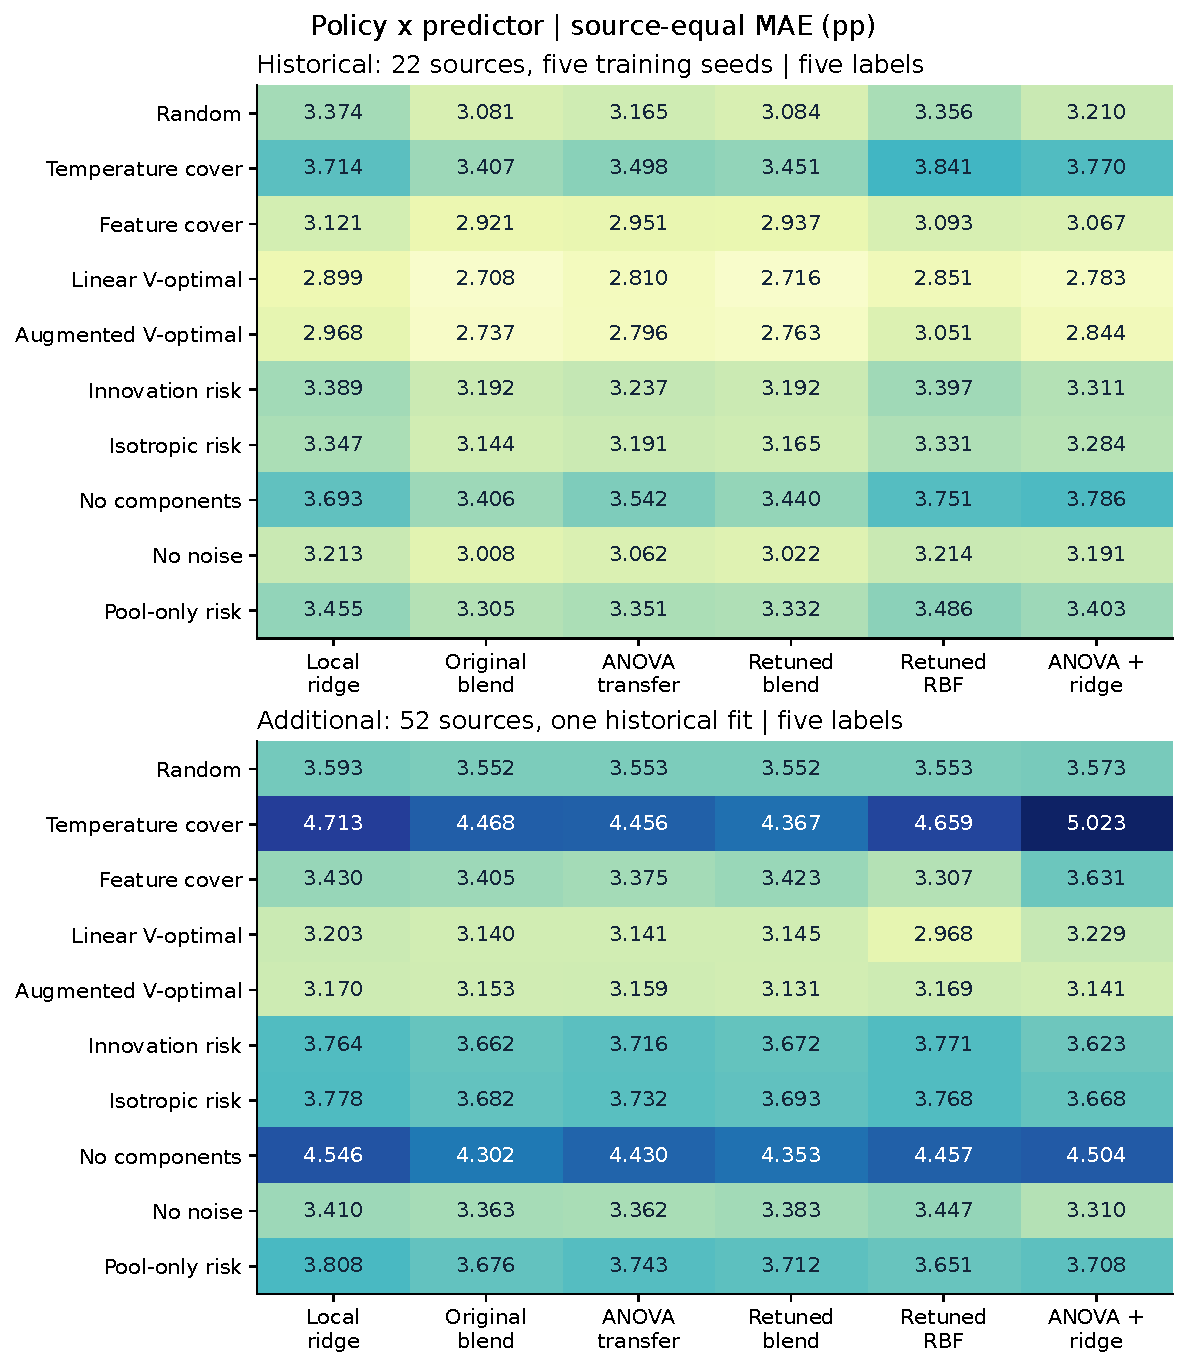
\includegraphics[width=\linewidth]{../figures/step5_01_factorial.pdf}\caption{Selected columns of the complete acquisition factorial at five labels. The following tables retain all thirteen predictors and ten policies.}\end{figure}
\begin{figure}[htbp]\centering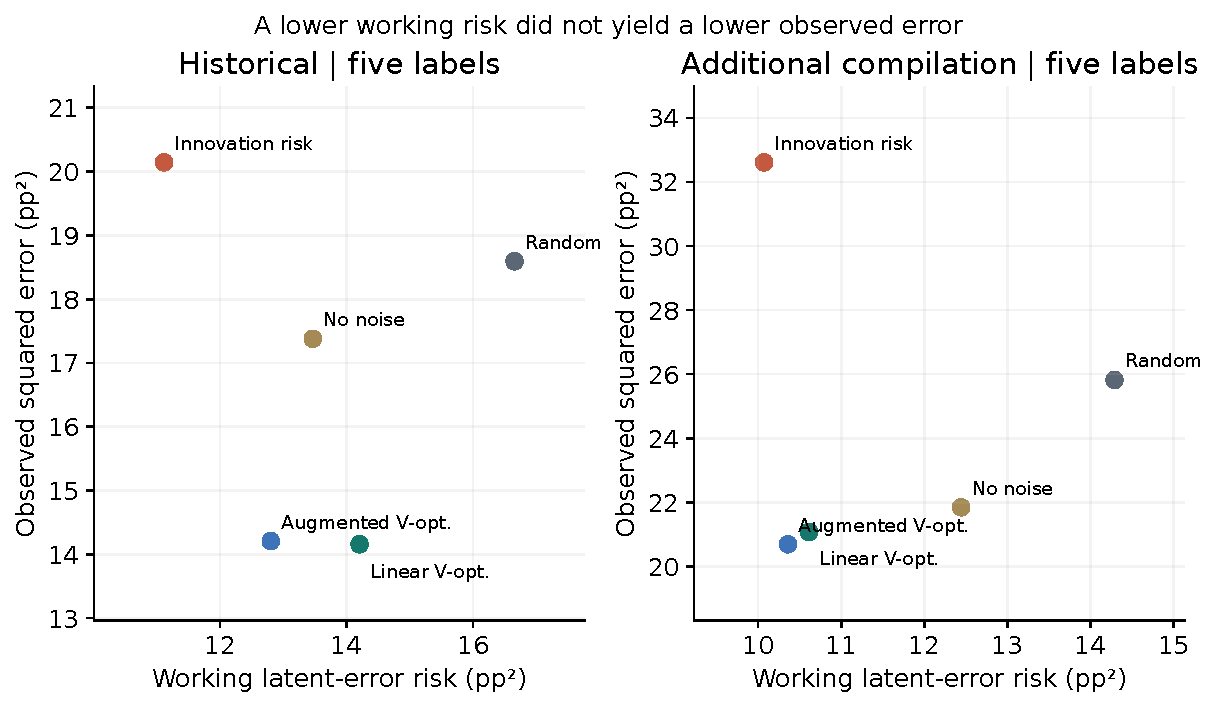
\includegraphics[width=\linewidth]{../figures/step5_04_risk_calibration.pdf}\caption{Secondary risk-calibration diagnostic for the fixed-prior predictor. Latent working risk excludes irreducible query noise; observed squared errors include outcome variability. Within a source, this support-independent noise cannot explain the full ordering discrepancy.}\end{figure}

\clearpage\begin{landscape}\begin{table}[htbp]\centering\small
\caption{Historical random queries, 22 sources. Five-label MAE (pp), all factors.}
\begin{tabular}{lrrrrrrrrrr}\toprule Predictor & R & T & F & L & A & I & S & NC & NN & P\\\midrule
Global & 4.527 & 4.527 & 4.527 & 4.527 & 4.527 & 4.527 & 4.527 & 4.527 & 4.527 & 4.527\\
Support mean & 3.693 & 3.935 & 3.491 & 3.409 & 3.497 & 3.672 & 3.666 & 3.947 & 3.709 & 3.775\\
Local ridge & 3.374 & 3.714 & 3.121 & 2.899 & 2.968 & 3.389 & 3.347 & 3.693 & 3.213 & 3.455\\
Original blend & 3.081 & 3.407 & 2.921 & 2.708 & 2.737 & 3.192 & 3.144 & 3.406 & 3.008 & 3.305\\
ANOVA transfer & 3.165 & 3.498 & 2.951 & 2.810 & 2.796 & 3.237 & 3.191 & 3.542 & 3.062 & 3.351\\
ANOVA fixed prior & 3.162 & 3.452 & 2.986 & 2.803 & 2.831 & 3.264 & 3.205 & 3.465 & 3.064 & 3.362\\
Local RBF & 3.356 & 3.755 & 3.143 & 2.899 & 3.047 & 3.435 & 3.370 & 3.720 & 3.256 & 3.484\\
2-component augmented & 3.127 & 3.521 & 3.028 & 2.718 & 2.736 & 3.239 & 3.190 & 3.524 & 3.067 & 3.313\\
Same-alpha residual & 3.171 & 3.420 & 2.961 & 2.802 & 2.795 & 3.261 & 3.150 & 3.462 & 3.032 & 3.389\\
Retuned local & 3.374 & 4.011 & 3.114 & 2.823 & 3.046 & 3.355 & 3.332 & 3.750 & 3.319 & 3.492\\
Retuned blend & 3.084 & 3.451 & 2.937 & 2.716 & 2.763 & 3.192 & 3.165 & 3.440 & 3.022 & 3.332\\
Retuned RBF & 3.356 & 3.841 & 3.093 & 2.851 & 3.051 & 3.397 & 3.331 & 3.751 & 3.214 & 3.486\\
3-component augmented & 3.210 & 3.770 & 3.067 & 2.783 & 2.844 & 3.311 & 3.284 & 3.786 & 3.191 & 3.403\\
\bottomrule\end{tabular}\par\medskip\footnotesize R: random; T: temperature cover; F: feature cover; L: linear V-optimal; A: augmented V-optimal; I: innovation risk; S: isotropic risk; NC: no components; NN: no noise; P: pool-only risk. Each column shares supports across predictors.\end{table}\end{landscape}

\clearpage\begin{landscape}\begin{table}[htbp]\centering\small
\caption{Additional random queries, 52 sources. Five-label MAE (pp), all factors.}
\begin{tabular}{lrrrrrrrrrr}\toprule Predictor & R & T & F & L & A & I & S & NC & NN & P\\\midrule
Global & 6.120 & 6.120 & 6.120 & 6.120 & 6.120 & 6.120 & 6.120 & 6.120 & 6.120 & 6.120\\
Support mean & 4.490 & 5.665 & 4.444 & 4.106 & 4.200 & 4.279 & 4.154 & 5.122 & 4.434 & 4.644\\
Local ridge & 3.593 & 4.713 & 3.430 & 3.203 & 3.170 & 3.764 & 3.778 & 4.546 & 3.410 & 3.808\\
Original blend & 3.552 & 4.468 & 3.405 & 3.140 & 3.153 & 3.662 & 3.682 & 4.302 & 3.363 & 3.676\\
ANOVA transfer & 3.553 & 4.456 & 3.375 & 3.141 & 3.159 & 3.716 & 3.732 & 4.430 & 3.362 & 3.743\\
ANOVA fixed prior & 3.553 & 4.456 & 3.375 & 3.141 & 3.159 & 3.716 & 3.732 & 4.430 & 3.362 & 3.743\\
Local RBF & 3.553 & 4.674 & 3.307 & 2.968 & 2.961 & 3.558 & 3.679 & 4.457 & 3.233 & 3.651\\
2-component augmented & 3.556 & 4.752 & 3.463 & 3.129 & 3.113 & 3.650 & 3.684 & 4.513 & 3.321 & 3.671\\
Same-alpha residual & 3.716 & 4.351 & 3.501 & 3.252 & 3.269 & 3.747 & 3.762 & 4.516 & 3.429 & 3.797\\
Retuned local & 3.593 & 4.713 & 3.455 & 3.155 & 3.170 & 3.764 & 3.778 & 4.546 & 3.410 & 3.808\\
Retuned blend & 3.552 & 4.367 & 3.423 & 3.145 & 3.131 & 3.672 & 3.693 & 4.353 & 3.383 & 3.712\\
Retuned RBF & 3.553 & 4.659 & 3.307 & 2.968 & 3.169 & 3.771 & 3.768 & 4.457 & 3.447 & 3.651\\
3-component augmented & 3.573 & 5.023 & 3.631 & 3.229 & 3.141 & 3.623 & 3.668 & 4.504 & 3.310 & 3.708\\
\bottomrule\end{tabular}\par\medskip\footnotesize R: random; T: temperature cover; F: feature cover; L: linear V-optimal; A: augmented V-optimal; I: innovation risk; S: isotropic risk; NC: no components; NN: no noise; P: pool-only risk. Each column shares supports across predictors.\end{table}\end{landscape}

\clearpage
\section{Source-contrast covariance transfer and matching acquisition}
\subsection{Why change the uncertainty model?}
The earlier acquisition risk identity is mathematically correct under its stated working model, but its empirical ordering does not track observed errors well. This is motivation for a distinct candidate, not an identified diagnosis of which earlier assumption failed. The present model directly describes cross-fitted errors of $\gamma f_G$ after removing source levels. It combines existing random-coefficient regression, a flat intercept, functional-response features and a matching integrated-variance objective. None of empirical Bayes, universal kriging, cross-fitting or V-optimality alone is an originality claim.

\subsection{Feature scaling and contrast records}
For historical source $s$ with at least 15 compatible rows, the unscaled feature vector contains the six preprocessed operating covariates and three ANOVA response functions. Each row's backbone, preprocessing and ANOVA reference set excludes that row's leakage group. Let $a_j=S^{-1}\sum_s\operatorname{mean}_i \phi_{sij}$ and $d_j^2=S^{-1}\sum_s\operatorname{mean}_i\phi_{sij}^2-a_j^2$, floored at $10^{-8}$. Divide by $d_j$; an additional subtraction of $a_j$ is unnecessary because the unrestricted source intercept makes joint feature translations irrelevant. Operating-only covariance uses the first six dimensions. All other variants use nine. These semantic coordinates allow three OOF dictionaries with different composition vocabularies to be combined without merging their full encoded feature vectors.

An outer historical fit has three first-level source-group folds. In tuning fold $j$, the whole held fold is absent from the covariance corpus. Within its complement, three new source-group folds supply OOF predictions for covariance rows. This requires nine secondary backbones per outer fit. Direct in-sample records from the same allowed complement form the in-sample ablation. The final deployment covariance uses the original three first-level OOF dictionaries on the complete historical training set. A fresh full historical fit reproduces the preceding full-fit geometry to numerical precision. The actual outer query groups, additional-publication outcomes and their labels never enter these fits.

\subsection{Stabilized posterior-moment estimation}
Define $X_s=\Phi_s-\mathbf1\overline\phi_s^\top$ and
$t_s=(y_s-\gamma f_{G,s})-\mathbf1\operatorname{mean}(y_s-\gamma f_{G,s})$.
The working prior is zero-mean with covariance $B$. Given current $B$ and $\sigma^2$,
\begin{align}
V_s&=(B^{-1}+X_s^\top X_s/\sigma^2)^{-1},\\
m_s&=V_sX_s^\top t_s/\sigma^2,\\
\widetilde B&=S^{-1}\sum_s(V_s+m_sm_s^\top),\\
\sigma_{\rm next}^2&=\frac{\sum_s[\|t_s-X_sm_s\|^2+\operatorname{tr}(X_s^\top X_sV_s)]}{\sum_s(n_s-1)}.
\end{align}
The full/operating/in-sample variants set $B_{\rm next}=0.8\widetilde B+0.2\operatorname{diag}(\widetilde B)$; diagonal keeps only its diagonal, and isotropic sets $B_{\rm next}=\operatorname{tr}(\widetilde B)I/p$. Eigendecomposition symmetrizes $B$ and floors its eigenvalues. With $v=\max[S^{-1}\sum_s\operatorname{mean}(t_s^2),10^{-6}]$, initialize $B=vI/p$ and $\sigma^2=v/2$. The common positive floor is $\max(v\times10^{-6},10^{-8})$. Stop after 80 updates or maximum relative covariance/noise change below $10^{-5}$. Every iteration count and final change is released. The procedure is a shrunk posterior-moment fit, not a proven exact REML maximum-likelihood optimizer. Noise pools contrast degrees of freedom, whereas covariance averages posterior second moments per source. Source-equal fitting of every variance term is not claimed.

For each variant, nine pairs $(\gamma,\eta)$ are assessed using ten random pseudo-support orders and budgets $1,2,3,5,10$. MAEs are first averaged over random orders, then equally over budgets and pseudo-sources. The minimum selects one pair for every budget and policy. The final covariance is refitted to allowed historical records at that gamma. This stage's pseudo-query scores are optimization diagnostics. Backbone configuration and original standard-design regularizers are inherited, not independently nested again through a new global configuration search.

\subsection{Established posterior and its information boundary}
The main-text posterior follows the GP with an explicit constant basis and an infinitely diffuse intercept prior \cite{gpml}. In a coefficient formulation, eliminating the intercept gives
\[
V_A=\left[B^{-1}+\frac{\Phi_{A,c}^\top\Phi_{A,c}}{\nu}\right]^{-1},\qquad
m_A=V_A\Phi_{A,c}^\top(r_A-\overline r_A\mathbf1)/\nu.
\]
The predictor is $\gamma f_{G,Q}+\overline r_A+(\Phi_Q-\overline\phi_A)m_A$. For $B=\tau^2I$ this is residual ridge with an unpenalized intercept and $\alpha=\nu/\tau^2$. Thus the isotropic version is an ordinary ridge working model; its mean transfer and its learned feature scaling are also explicit parts of the comparator.

The data information increment is $\Phi_{A,c}^\top\Phi_{A,c}/\nu$, with rank at most $\min(p,k-1)$. A component constant over supports has no independent contrast information. Off-diagonal prior covariance can couple its posterior update to observed directions, but those relationships originate in historical data, not new independent target labels. Bayesian conditioning cannot manufacture missing target information. At one label the posterior coefficient mean is zero and the prediction uses a global-response increment plus the estimated source offset.

With frozen working hyperparameters, additional support observations cannot increase latent posterior covariance in positive-semidefinite order; the flat-intercept limit is well defined for nonempty supports and positive noise. Consequently, the integrated-variance criterion is nonincreasing along the nested greedy sequence. Greedy selection need not be globally optimal, nor does decreasing working variance imply decreasing real MAE. The observation predictor's working variance adds $\nu$ to the latent diagonal. Neither variance includes uncertainty in estimated $B$, gamma, feature dictionary or inherited backbone choice.

\subsection{Controls and statistical estimands}
Policies are random, inherited linear V-optimal, inherited ANOVA-augmented V-optimal, contrast V-optimal, and contrast pool-only. Candidate pools and query rows are identical across rules. The two standard-design orders are exactly reproduced using the preceding regularizers and component scales. The contrast rule sees known query features; pool-only does not. Random is evaluated with 50 orders per source, deterministic rules once. All predictors share each policy's labels.

The eight noncandidate predictors are global, support mean, frozen local ridge, frozen original blend, re-tuned blend, re-tuned local ridge, re-tuned RBF, and ordinary ANOVA-feature ridge. Re-tuned ridge/residual controls use $\alpha\in\{0.1,1,10,100\}$. RBF uses the preceding nine $(\alpha,\gamma_{\rm RBF})$ combinations. Ordinary ANOVA ridge uses inherited component scales and four alphas. Stronger blend controls first select separate local/residual alphas by source-equal pseudo-query MAE, then select a prior weight in $\{0,0.25,0.5,0.75,1\}$ and shrinkage in $\{\infty,10,2,0.5,0\}$; its evidence scale remains inherited. These controls are tuned separately per policy/budget, whereas every covariance variant keeps one random-tuned pair across all budgets/policies.

All evaluation MAEs first average orders within each source/seed, then seeds within source, then sources. Publication leakage groups are resampled in 20,000 bootstrap draws. Intervals condition on fitted models. The four locked random-query $k=5$ comparisons are contrast-design/contrast-predictor versus linear-design/re-tuned-blend; versus augmented-design/re-tuned-blend; versus contrast-design/re-tuned-blend; and versus augmented-design/the same contrast predictor. Bonferroni percentile tails are $0.05/(2\times4)$ and their complement, adjusted separately within each cohort. All additional contrasts are exploratory. Prior inspection of the same corpora remains a limitation despite this within-stage protocol lock.

Support permutation is a descriptive mechanism diagnostic using repeat-zero five-label supports, twenty permutations per cell. It preserves the support mean but removes its response--input assignment. It does not estimate prospective deployment error, identify causal catalysis mechanisms or add independent sources.

\subsection{Observed performance, matched ablations and verification}
\begin{figure}[htbp]\centering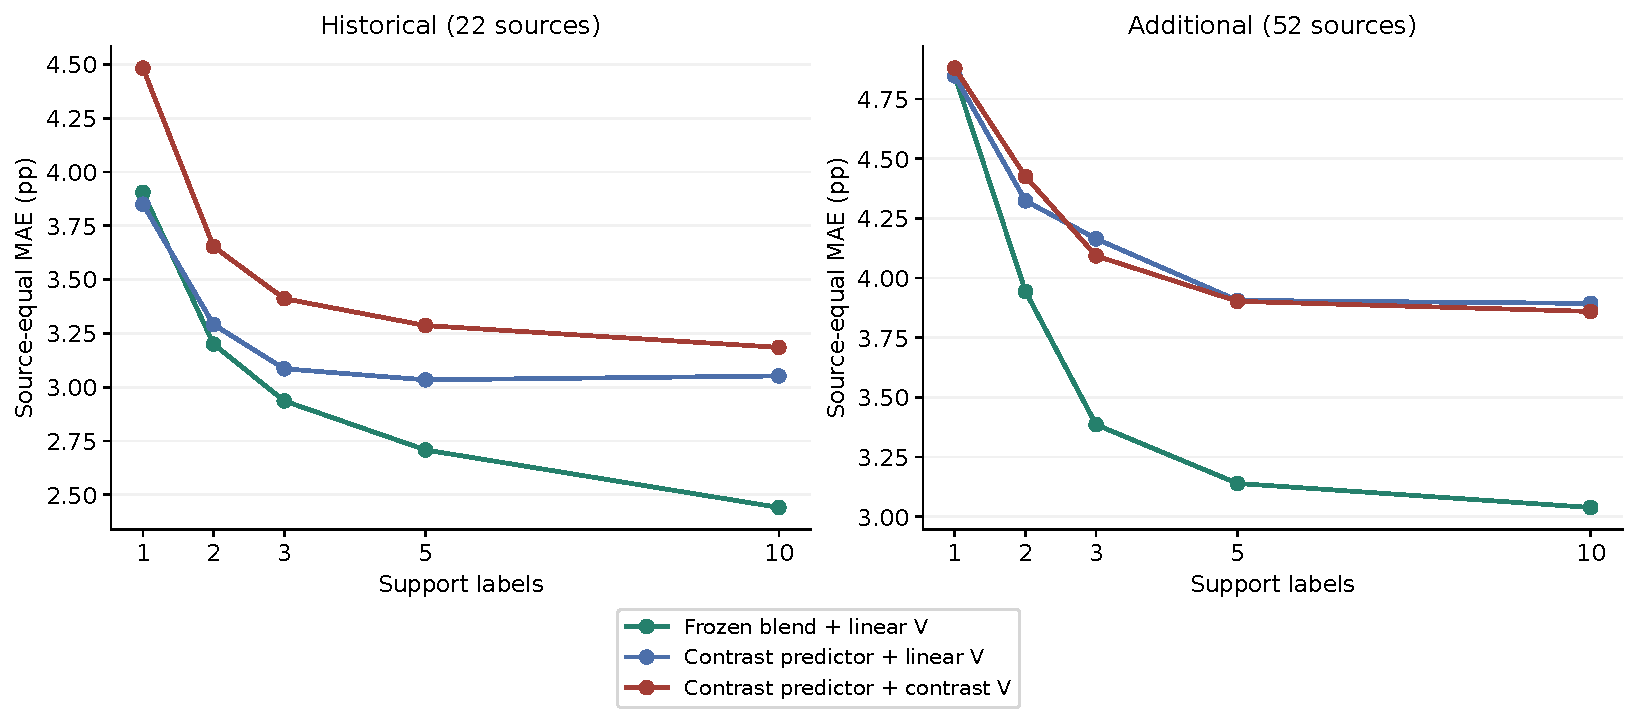
\includegraphics[width=\linewidth]{../figures/step6_02_budgets.pdf}\caption{Random-query budgets with fixed source populations. Standard-design frozen blending remains a comparator at every budget; no curve is selected using additional-source outcomes.}\end{figure}
\begin{figure}[htbp]\centering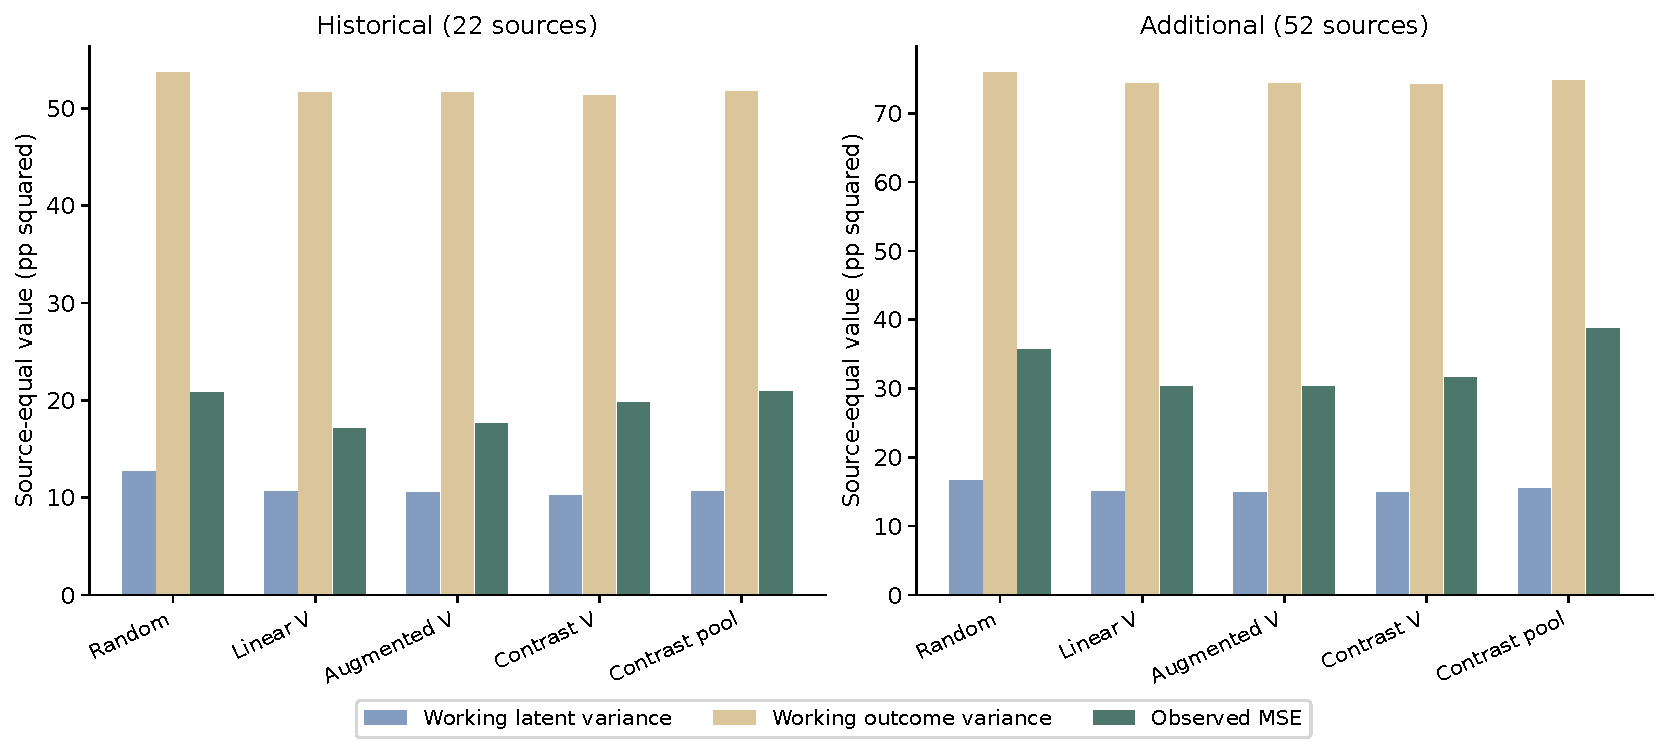
\includegraphics[width=\linewidth]{../figures/step6_03_variance_diagnostic.pdf}\caption{Five-label working variances versus observed MSE. Observation variance adds the frozen working residual term; this term includes lack of fit. These averages do not certify predictive coverage or identify physical laboratory noise.}\end{figure}
\FloatBarrier
\begin{table}[htbp]\centering\small\caption{Historical, 22 sources. Five-label random-query MAE (pp), all 65 factors.}\begin{tabular}{lrrrrr}\toprule Predictor & R & L & A & C & P\\\midrule
Global & 4.527 & 4.527 & 4.527 & 4.527 & 4.527\\
Support mean & 3.693 & 3.409 & 3.497 & 3.624 & 3.675\\
Frozen local ridge & 3.374 & 2.899 & 2.968 & 3.196 & 3.300\\
Frozen blend & 3.081 & 2.708 & 2.737 & 2.920 & 3.030\\
Retuned blend & 3.073 & 2.696 & 2.897 & 3.027 & 3.080\\
Retuned local ridge & 3.374 & 2.823 & 3.046 & 3.304 & 3.297\\
Retuned RBF & 3.356 & 2.851 & 3.051 & 3.303 & 3.222\\
Ordinary ANOVA ridge & 3.210 & 2.783 & 2.844 & 3.129 & 3.230\\
Contrast full & 3.365 & 3.034 & 3.090 & 3.287 & 3.389\\
Contrast diagonal & 3.368 & 3.049 & 3.096 & 3.296 & 3.390\\
Operating only & 3.430 & 3.064 & 3.153 & 3.340 & 3.452\\
Isotropic & 3.390 & 3.059 & 3.107 & 3.300 & 3.413\\
In-sample covariance & 3.382 & 3.065 & 3.063 & 3.291 & 3.369\\
\bottomrule\end{tabular}\par\smallskip\footnotesize R: random; L: linear V-optimal; A: augmented V-optimal; C: contrast V-optimal; P: contrast pool-only. All columns share query populations; each column shares supports across predictors.\end{table}
\begin{table}[htbp]\centering\small\caption{Additional, 52 sources. Five-label random-query MAE (pp), all 65 factors.}\begin{tabular}{lrrrrr}\toprule Predictor & R & L & A & C & P\\\midrule
Global & 6.120 & 6.120 & 6.120 & 6.120 & 6.120\\
Support mean & 4.490 & 4.106 & 4.200 & 4.015 & 4.290\\
Frozen local ridge & 3.593 & 3.203 & 3.170 & 3.447 & 3.744\\
Frozen blend & 3.552 & 3.140 & 3.153 & 3.411 & 3.710\\
Retuned blend & 3.571 & 3.149 & 3.157 & 3.422 & 3.619\\
Retuned local ridge & 3.593 & 3.155 & 3.170 & 3.447 & 3.744\\
Retuned RBF & 3.553 & 2.968 & 3.169 & 3.478 & 3.744\\
Ordinary ANOVA ridge & 3.573 & 3.229 & 3.141 & 3.349 & 3.709\\
Contrast full & 4.298 & 3.907 & 4.003 & 3.903 & 4.184\\
Contrast diagonal & 4.338 & 3.952 & 4.050 & 3.920 & 4.201\\
Operating only & 4.405 & 4.032 & 4.114 & 3.981 & 4.280\\
Isotropic & 3.936 & 3.589 & 3.617 & 3.753 & 3.995\\
In-sample covariance & 4.231 & 3.802 & 3.833 & 3.927 & 4.206\\
\bottomrule\end{tabular}\par\smallskip\footnotesize R: random; L: linear V-optimal; A: augmented V-optimal; C: contrast V-optimal; P: contrast pool-only. All columns share query populations; each column shares supports across predictors.\end{table}
\FloatBarrier\begin{table}[htbp]\centering\small\caption{Post-hoc parameter-matched covariance diagnostic. Linear-design supports at five labels; gamma and total observation noise are fixed to the main candidate. Nominal intervals are exploratory.}\begin{tabular}{lrr}\toprule Covariance & Historical MAE & Additional MAE\\\midrule
Contrast full & 3.034 & 3.907\\
Contrast diagonal & 3.040 & 3.951\\
Operating only & 3.054 & 4.027\\
Isotropic & 3.048 & 3.823\\
In-sample covariance & 3.045 & 3.982\\
\bottomrule\end{tabular}\end{table}
The candidate's historical dictionary has nine dimensions, whereas full-feature local ridge/RBF uses six operating features plus historical composition vocabulary channels. The covariance ablations are cleaner tests of covariance choices than the comparison with those wider dictionaries; neither supplies a unique causal explanation for failure. Independently tuned variants may choose different gammas/noise multipliers. The matched diagnostic was added after the locked results were observed, uses the main historical gamma and total noise, and makes no new selection from query outcomes. It evaluates all five covariance alternatives, including unfavorable ones.

The complete stage contains 61290 error cells, 65 predictor--policy combinations, and five new covariance-transfer variants. All 11,804 inherited support orders and 236,080 original-method MAEs reproduce the preceding stage to maximum $3.56\times10^{-15}$. The covariance stage refits 338 backbones in total: 26 full, 78 first-level and 234 secondary. The released numerical verifier checks isotropic-ridge equivalence, feature/response shift identities, all ten greedy steps against scalar scores, constant-feature nonidentifiability, and a 100,000-trial Gaussian risk simulation (0.311\% relative error). Independent row audits and poisoned-outcome support-order checks are archived with exact counts. Prediction files are lossless float64 NPZ, without object arrays or quantization.

The sixth release's covariance entry point re-fits Section 13; it does not claim to newly re-fit all earlier multi-task studies. Full covariance records and arrays remain in that sixth release. The seventh release preserves the covariance summaries and figures but re-fits the separate cross-task acquisition experiment in Section 14. A separate fresh-directory smoke check re-fits one historical regime from an extracted package; the full mode re-fits all 26. Manifest verification and numerical audit use released outputs without treating a completed cache as a new training run.

\section{Cross-task standard acquisition extension}
\subsection{Scope, chronology and fixed populations}
This seventh extension evaluates five panels from four outcomes in two reaction systems, not five independent reaction datasets. Conversion and selectivity share the same paired records; twenty publication identifiers overlap the STY collection; OCM F0/F1 use the same records. These dependencies remain relevant when interpreting breadth. The current protocol is timestamped and hashed before current outer evaluation, but all input corpora were already inspected in earlier development. All new results are retrospective. Only the five-label frozen-blend query-V-minus-random comparison across the five random-query panels is primary. The parameter-matched OCM geometry crossing was added after primary results and is explicitly exploratory.

Every outer seed/fold and backbone configuration is inherited verbatim from the preceding full-study benchmark. Current outer models are re-fitted and compared with the original zero-label predictions. Historical source-disjoint OOF responses are reused for policy-specific control tuning. Inner preprocessors are reconstructed using the same three historical training-group partitions; no pseudo-validation group fits its own feature preprocessor. There is no new inner backbone fit or new global-configuration search in this extension. OOF model configuration was selected within the complete outer historical-training set in the earlier benchmark; historical control scores remain optimization diagnostics, not independent test results. Outer query groups are excluded from every such choice.

Random queries, high-temperature queries and reported-stratum holdouts use the original label-blind definitions. Eligibility is unchanged: at least ten pool records, at least five query records. Pool IDs are sorted before selection. Deterministic acquisitions are evaluated once, rather than copied fifty times as artificial replicates. Random orders run fifty times. Every policy produces one nested sequence to budget ten; intermediate steps use the original local-ridge alpha of the next reported budget. Different target outcomes can have different frozen alpha schedules, even when they share feature rows.

\subsection{Five acquisitions and thirteen predictors}
Temperature coverage uses the first numeric feature; full-feature coverage uses all allowed standardized/imputed numeric and encoded-composition features. The first row is nearest the pool mean and later rows maximize their minimum squared distance to the selected set. This is a conventional coverage heuristic. Query and pool V-optimal acquisition use a unit linear coefficient prior on $[10,z]$ and the inherited random-design local alpha. Query V minimizes mean working posterior variance on query covariates; pool V minimizes it over all candidate-pool covariates, including candidates that may later be observed. Neither reads outcomes. The finite intercept prior used for acquisition differs from the exact unpenalized intercept used for prediction, so working variance is only a design surrogate.

Nine original predictors are frozen: global, support mean, residual offset, affine, empirical Bayes, local ridge, temperature ridge, residual ridge and shrinkage blend. Four stronger controls re-tune local ridge, residual ridge, blending and local RBF by policy/budget. Ridge alphas are $\{0.1,1,10,100\}$. RBF alpha and gamma both use $\{0.01,0.1,1\}$ and $\{0.1,1,10\}$, respectively; squared distances divide by feature dimension. Kernel ridge centers its support kernel and response and restores the support mean. After local/residual alpha selection, blending evaluates five prior weights times five shrinkages, using the inherited response scale and support-only analytic LOO. Each candidate's MAE is averaged over historical support draws, then pseudo-sources. Random pseudo-supports repeat ten times; deterministic policies once. All control grids and acquired rows are common across policies. An ordinary kernel/local fit is a strong comparator; a lower point estimate is not selected using outer query outcomes.

\subsection{Primary family, units and aggregation}
Each error cell averages query rows, then repeated support draws are averaged within source/seed, then seeds within source, then sources receive equal weight. A leakage group may contain more than one source; cluster bootstrap retains those source weights. Twenty thousand group resamples produce nominal 95\% intervals. Five-panel primary tails are 0.005 and 0.995, the approximate Bonferroni-adjusted 99\% percentile interval. Adjustment accommodates endpoint dependence but does not include training-fit uncertainty or remove retrospective selection. No folds, random draws, or shuffled-label draws are counted as independent publications. STY uses its native productivity unit, while the other outcomes use percentage points; raw errors are not pooled across these units.

\begin{table}[htbp]\centering\small\caption{Five-panel adjusted primary results. Same interpretation and units as the main primary table.}\begin{tabular}{lrrrrl}\toprule Panel & $n$ & Random & Query V & Gain (\%) & Adjusted $\Delta$ interval\\\midrule
Conversion & 32 & 2.441 & 2.121 & 13.1 & [-0.707, 0.068]\\
Selectivity & 32 & 11.584 & 10.683 & 7.8 & [-2.140, 0.615]\\
STY & 28 & 62.608 & 50.274 & 19.7 & [-25.965, -2.874]\\
OCM F0 & 22 & 3.660 & 3.768 & -3.0 & [-0.355, 0.714]\\
OCM F1 & 22 & 3.081 & 2.708 & 12.1 & [-0.746, -0.056]\\
\bottomrule\end{tabular}
\end{table}
\begin{table}[htbp]\centering\small\caption{Frozen blend across five acquisitions at five labels. R: random; T: temperature coverage; F: feature coverage; V: query V; P: pool V. STY has native productivity units; other rows are percentage points.}\begin{tabular}{lrrrrr}\toprule Panel & R & T & F & V & P\\\midrule
Conversion & 2.441 & 2.647 & 2.172 & 2.121 & 2.417\\
Selectivity & 11.584 & 13.606 & 11.096 & 10.683 & 10.481\\
STY & 62.608 & 70.661 & 53.111 & 50.274 & 58.440\\
OCM F0 & 3.660 & 3.901 & 4.008 & 3.768 & 3.895\\
OCM F1 & 3.081 & 3.407 & 2.921 & 2.708 & 2.886\\
\bottomrule\end{tabular}
\end{table}
\FloatBarrier\begin{figure}[htbp]\centering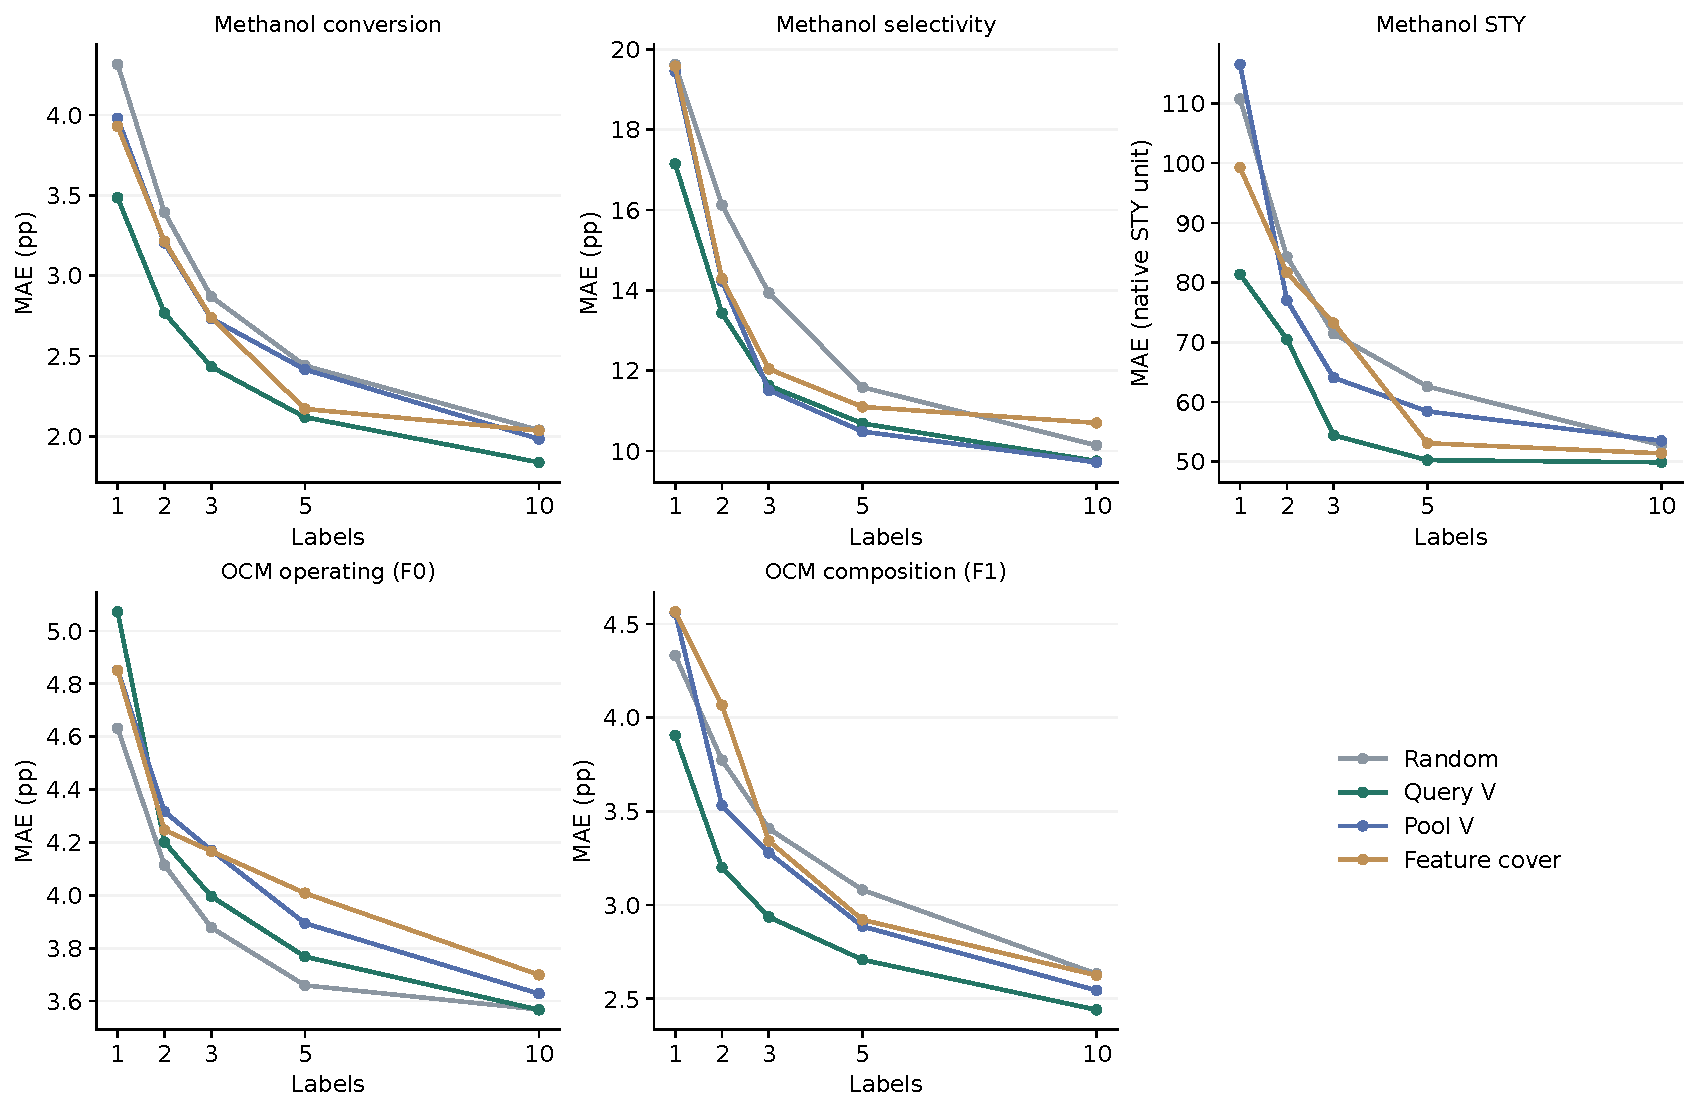
\includegraphics[width=\linewidth]{../figures/step7_02_budgets.pdf}\caption{Budget curves for the unchanged frozen blend on five random-query panels. All rules share each panel's query population. The four displayed rules are representative; all five acquisitions and thirteen predictors are available in the numerical tables.}\end{figure}\FloatBarrier

\begin{table}[htbp]\centering\small
\caption{Methanol conversion: all five-label random-query factors. Native STY units for STY; percentage points otherwise.}
\begin{tabular}{lrrrrr}\toprule Predictor & R & T & F & V & P\\\midrule
Global & 5.271 & 5.271 & 5.271 & 5.271 & 5.271\\
Support mean & 4.304 & 4.182 & 4.063 & 3.806 & 4.315\\
Offset & 3.455 & 3.459 & 3.376 & 3.226 & 3.539\\
Affine & 3.083 & 3.239 & 2.926 & 2.839 & 3.098\\
Empirical Bayes & 3.457 & 3.437 & 3.383 & 3.242 & 3.506\\
Frozen local ridge & 2.429 & 2.576 & 2.197 & 2.135 & 2.394\\
Temperature ridge & 2.519 & 2.711 & 2.470 & 2.343 & 2.587\\
Frozen residual ridge & 2.720 & 2.873 & 2.540 & 2.395 & 2.669\\
Frozen blend & 2.441 & 2.647 & 2.172 & 2.121 & 2.417\\
Retuned local ridge & 2.429 & 2.647 & 2.271 & 2.173 & 2.472\\
Retuned residual ridge & 2.720 & 2.856 & 2.524 & 2.421 & 2.668\\
Retuned blend & 2.421 & 2.633 & 2.187 & 2.120 & 2.407\\
Retuned local RBF & 2.401 & 2.531 & 2.075 & 2.153 & 2.436\\
\bottomrule\end{tabular}\par\smallskip\footnotesize R: random; T: temperature cover; F: feature cover; V: query V-optimal; P: pool V-optimal. Supports are common across predictors within a policy.\end{table}\FloatBarrier
\begin{table}[htbp]\centering\small
\caption{Methanol selectivity: all five-label random-query factors. Native STY units for STY; percentage points otherwise.}
\begin{tabular}{lrrrrr}\toprule Predictor & R & T & F & V & P\\\midrule
Global & 22.740 & 22.740 & 22.740 & 22.740 & 22.740\\
Support mean & 17.136 & 16.999 & 16.998 & 15.806 & 17.521\\
Offset & 15.747 & 16.207 & 16.310 & 15.126 & 16.275\\
Affine & 12.539 & 12.520 & 12.214 & 11.842 & 12.014\\
Empirical Bayes & 15.988 & 16.439 & 16.481 & 15.424 & 16.501\\
Frozen local ridge & 11.547 & 12.689 & 11.142 & 10.725 & 10.568\\
Temperature ridge & 11.535 & 11.561 & 11.626 & 10.973 & 11.299\\
Frozen residual ridge & 12.077 & 14.678 & 11.332 & 10.735 & 10.850\\
Frozen blend & 11.584 & 13.606 & 11.096 & 10.683 & 10.481\\
Retuned local ridge & 11.547 & 12.381 & 11.336 & 10.762 & 10.568\\
Retuned residual ridge & 12.077 & 13.917 & 11.102 & 10.790 & 10.793\\
Retuned blend & 11.623 & 12.159 & 11.097 & 10.691 & 10.579\\
Retuned local RBF & 11.122 & 11.201 & 10.774 & 10.558 & 10.231\\
\bottomrule\end{tabular}\par\smallskip\footnotesize R: random; T: temperature cover; F: feature cover; V: query V-optimal; P: pool V-optimal. Supports are common across predictors within a policy.\end{table}\FloatBarrier
\begin{table}[htbp]\centering\small
\caption{Methanol STY: all five-label random-query factors. Native STY units for STY; percentage points otherwise.}
\begin{tabular}{lrrrrr}\toprule Predictor & R & T & F & V & P\\\midrule
Global & 139.258 & 139.258 & 139.258 & 139.258 & 139.258\\
Support mean & 91.993 & 110.199 & 101.256 & 77.514 & 97.591\\
Offset & 88.265 & 104.855 & 92.493 & 78.964 & 90.901\\
Affine & 71.225 & 82.290 & 69.447 & 62.853 & 71.968\\
Empirical Bayes & 86.510 & 98.390 & 90.549 & 78.972 & 88.594\\
Frozen local ridge & 65.210 & 72.805 & 56.486 & 52.671 & 61.580\\
Temperature ridge & 87.098 & 96.672 & 86.843 & 66.248 & 88.206\\
Frozen residual ridge & 69.889 & 76.255 & 62.666 & 57.442 & 65.811\\
Frozen blend & 62.608 & 70.661 & 53.111 & 50.274 & 58.440\\
Retuned local ridge & 65.210 & 69.453 & 56.283 & 51.293 & 60.031\\
Retuned residual ridge & 69.889 & 77.153 & 62.784 & 57.352 & 65.539\\
Retuned blend & 62.613 & 69.483 & 53.103 & 49.852 & 56.767\\
Retuned local RBF & 63.957 & 68.185 & 54.535 & 51.547 & 62.927\\
\bottomrule\end{tabular}\par\smallskip\footnotesize R: random; T: temperature cover; F: feature cover; V: query V-optimal; P: pool V-optimal. Supports are common across predictors within a policy.\end{table}\FloatBarrier
\begin{table}[htbp]\centering\small
\caption{OCM operating (F0): all five-label random-query factors. Native STY units for STY; percentage points otherwise.}
\begin{tabular}{lrrrrr}\toprule Predictor & R & T & F & V & P\\\midrule
Global & 5.302 & 5.302 & 5.302 & 5.302 & 5.302\\
Support mean & 3.693 & 3.935 & 4.038 & 3.802 & 3.907\\
Offset & 3.672 & 3.931 & 3.997 & 3.819 & 3.932\\
Affine & 3.694 & 3.933 & 4.005 & 3.796 & 3.941\\
Empirical Bayes & 3.759 & 3.963 & 4.000 & 3.866 & 3.956\\
Frozen local ridge & 3.655 & 3.905 & 4.027 & 3.754 & 3.877\\
Temperature ridge & 3.677 & 3.961 & 4.048 & 3.771 & 3.885\\
Frozen residual ridge & 3.701 & 3.930 & 4.012 & 3.799 & 3.948\\
Frozen blend & 3.660 & 3.901 & 4.008 & 3.768 & 3.895\\
Retuned local ridge & 3.655 & 4.006 & 4.111 & 3.776 & 3.908\\
Retuned residual ridge & 3.701 & 3.974 & 4.070 & 3.792 & 4.007\\
Retuned blend & 3.665 & 3.989 & 4.072 & 3.774 & 3.945\\
Retuned local RBF & 3.671 & 3.972 & 4.086 & 3.756 & 3.931\\
\bottomrule\end{tabular}\par\smallskip\footnotesize R: random; T: temperature cover; F: feature cover; V: query V-optimal; P: pool V-optimal. Supports are common across predictors within a policy.\end{table}\FloatBarrier
\begin{table}[htbp]\centering\small
\caption{OCM composition (F1): all five-label random-query factors. Native STY units for STY; percentage points otherwise.}
\begin{tabular}{lrrrrr}\toprule Predictor & R & T & F & V & P\\\midrule
Global & 4.527 & 4.527 & 4.527 & 4.527 & 4.527\\
Support mean & 3.693 & 3.935 & 3.491 & 3.409 & 3.688\\
Offset & 3.423 & 3.682 & 3.195 & 3.041 & 3.429\\
Affine & 3.360 & 3.564 & 3.193 & 2.976 & 3.365\\
Empirical Bayes & 3.415 & 3.645 & 3.227 & 3.120 & 3.366\\
Frozen local ridge & 3.374 & 3.714 & 3.121 & 2.899 & 3.109\\
Temperature ridge & 3.677 & 3.961 & 3.471 & 3.373 & 3.664\\
Frozen residual ridge & 3.109 & 3.332 & 2.940 & 2.759 & 2.927\\
Frozen blend & 3.081 & 3.407 & 2.921 & 2.708 & 2.886\\
Retuned local ridge & 3.374 & 4.011 & 3.114 & 2.823 & 3.114\\
Retuned residual ridge & 3.109 & 3.554 & 3.056 & 2.790 & 2.961\\
Retuned blend & 3.073 & 3.659 & 2.994 & 2.696 & 2.911\\
Retuned local RBF & 3.356 & 3.841 & 3.093 & 2.851 & 3.116\\
\bottomrule\end{tabular}\par\smallskip\footnotesize R: random; T: temperature cover; F: feature cover; V: query V-optimal; P: pool V-optimal. Supports are common across predictors within a policy.\end{table}\FloatBarrier

\subsection{Label-correspondence diagnostic}
At budget five, the first random order and each deterministic support are used for twenty outcome permutations per source/scenario/seed. The input rows, global predictions, support outcomes as a multiset, and exact support mean remain the same; only input--label correspondence changes. The frozen blend is re-computed, including its support-only blend weight. Query labels enter scoring only. These are exploratory controls, not repeated training datasets or a physical perturbation experiment. Permutation errors average shuffles and seeds before source-group intervals.

\begin{table}[htbp]\centering\small\caption{Correspondence shuffling under query V: frozen blend, five labels. Nominal source-group intervals are exploratory.}\begin{tabular}{lrrl}\toprule Panel & Aligned & Shuffled & Shuffled minus aligned, 95\% CI\\\midrule
Conversion & 2.121 & 4.135 & 2.015 [1.253, 2.851]\\
Selectivity & 10.683 & 16.723 & 6.040 [3.693, 8.513]\\
STY & 50.274 & 80.945 & 30.671 [10.436, 59.603]\\
OCM F0 & 3.768 & 3.815 & 0.047 [-0.009, 0.134]\\
OCM F1 & 2.708 & 3.548 & 0.840 [0.478, 1.237]\\
\bottomrule\end{tabular}\end{table}
\FloatBarrier\begin{figure}[htbp]\centering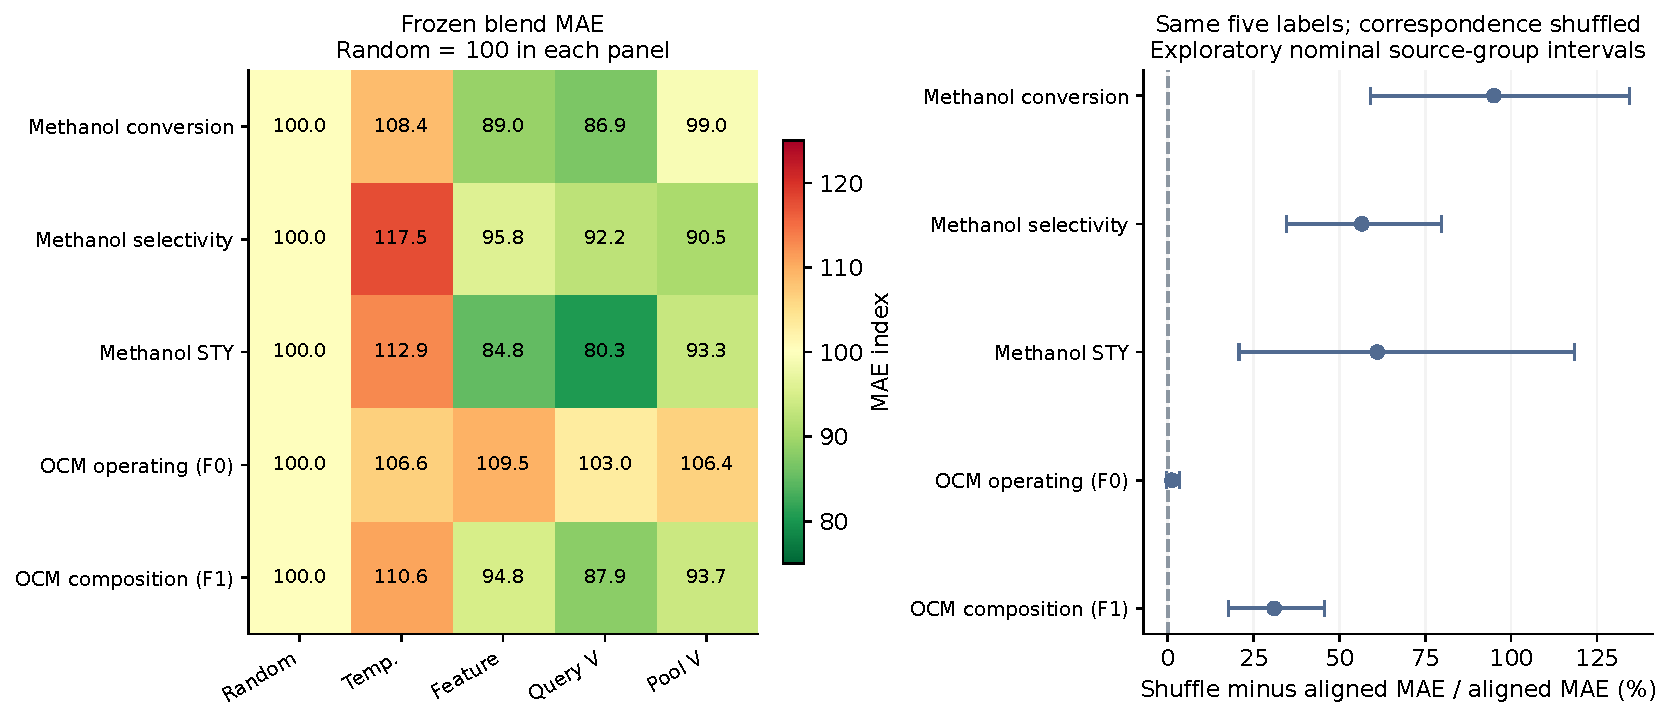
\includegraphics[width=\linewidth]{../figures/step7_03_information.pdf}\caption{Left: all acquisition means for the frozen blend, normalized to each panel's observed random-design MAE. Right: outcome-correspondence shuffling effect, nominal native-unit intervals rescaled by the fixed observed aligned MAE. Normalization is for display, not a pooled or bootstrap ratio estimand.}\end{figure}\FloatBarrier

\subsection{Post-primary representation crossing}
The OCM follow-up fixes the F1 alpha schedule for both operating-only (six-feature) and full composition-enriched V geometry. It evaluates each acquired sequence with both already frozen F0 and F1 predictors. Numeric preprocessors are verified equal between paired representations; outcomes, pool rows and queries are identical. The full-geometry orders exactly match the original F1 orders. The operating-only orders in this follow-up can differ from the primary F0 orders because the regularizer is now fixed to F1, rather than independently inherited from F0. A direct comparison of the primary F0 and F1 numbers would mix representation, backbone/adapter choices and acquisition regularization; this crossing removes the acquisition-alpha difference for its own conditional contrasts.

\begin{figure}[htbp]\centering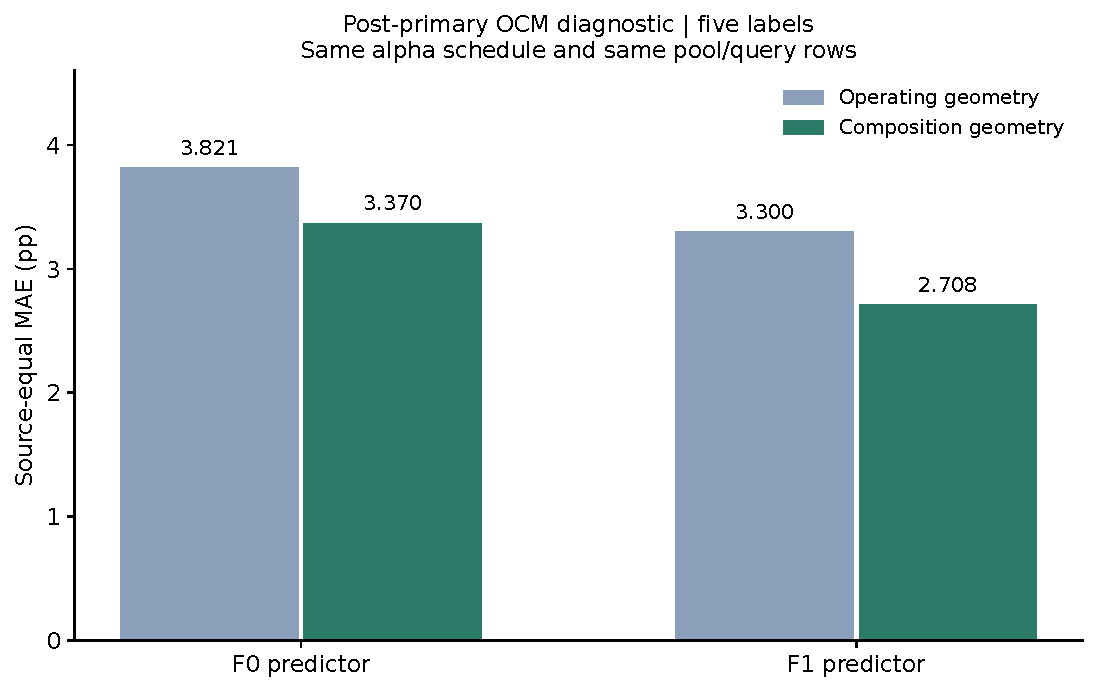
\includegraphics[width=.85\linewidth]{../figures/step7_04_geometry.pdf}\caption{Post-primary exploratory crossing of selection geometry and prediction representation. Same F1 alpha, five supports, 22 OCM sources. Geometry-specific nominal intervals and all budgets are released. No new training or parameter selection occurs. Composition used for acquisition is not automatically an input to the F0 predictor.}\end{figure}\FloatBarrier

\subsection{Independent verification and reproduction scope}
The current computation contains 125 outer fits, 330,750 error cells, 66,150 nested orders, and 31,712,850 scalar row predictions across 65 combinations per panel. Exactly 125 new outer backbones and zero new inner backbones are trained. Original random-design MAEs reproduce across 306,250 cells and nine methods, with maximum discrepancy 2.77e-09. The larger STY scale explains why this roundoff is not identical to the percentage-point panels. OCM frozen query/random orders and original four-method errors independently match the sixth release.

Independent audits re-aggregate 31,712,850 scalar predictions and reconstruct 2,936,375 from support rows. All 66,150 selection orders remain unchanged after replacing every target response by values between $-10^9$ and $10^9$. Five hundred outer/inner group-separation checks pass. Mathematical verification compares all twenty greedy steps of query/pool design with a direct primal posterior and checks exact ridge prediction/LOO against independent scikit-learn fits. The post-primary crossing adds 2,700 cells and 172,800 scalar predictions, with an independent read-only audit.

The seventh release includes lossless float64 NPZ predictions, acquired/query ID ledgers, historical control scores, every parameter, input snapshots, split ledgers, predecessor references and a checksummed manifest. Its verify mode reads the release and writes audit reports only into a temporary directory. Smoke mode re-fits one OCM F1 outer fold in an empty external directory; full mode re-fits all 125 current outer models, re-tunes the current controls from inherited historical OOF records and repeats the post-primary geometry diagnostic. A completed cache is never counted as a fresh refit. The smoke check is a portability check, not a second full 125-fit independent repetition. Earlier Section 1--13 studies retain their complete raw arrays in the prior numbered releases, rather than being claimed as newly re-run by the current entry point.


\begin{thebibliography}{12}\small
\bibitem{toldy} Toldy, \'A. I. et al. TheMeCat: Dataset of Thermocatalytic Conversion of CO$_2$ to Methanol. \emph{Scientific Data} \textbf{13}, 165 (2026). \url{https://doi.org/10.1038/s41597-025-06482-8}.
\bibitem{yan} Yan, M. et al. A machine learning perspective on three decades of methanol synthesis: research framework and experimental operation insights. \emph{Communications Engineering} \textbf{5}, 162 (2026). \url{https://doi.org/10.1038/s44172-026-00706-4}.
\bibitem{suvarna} Suvarna, M., Ara\'ujo, T. P. \& P\'erez-Ram\'irez, J. A generalized machine learning framework to predict the space-time yield of methanol from thermocatalytic CO$_2$ hydrogenation. \emph{Applied Catalysis B: Environmental} \textbf{315}, 121530 (2022). \url{https://doi.org/10.1016/j.apcatb.2022.121530}.
\bibitem{schmack} Schmack, R. et al. A meta-analysis of catalytic literature data reveals property--performance correlations for the OCM reaction. \emph{Nature Communications} \textbf{10}, 441 (2019). \url{https://doi.org/10.1038/s41467-019-08325-8}.
\bibitem{mine} Mine, S. et al. Analysis of Updated Literature Data up to 2019 on the Oxidative Coupling of Methane Using an Extrapolative Machine-Learning Method to Identify Novel Catalysts. \emph{ChemCatChem} (2021). \url{https://doi.org/10.1002/cctc.202100495}. Data: \url{https://github.com/mts-uw/OCM}, commit \texttt{dbf7be5aadb30323f825e8f7d7f6bd3012c99dd2}.
\bibitem{roberts} Roberts, D. R. et al. Cross-validation strategies for data with temporal, spatial, hierarchical, or phylogenetic structure. \emph{Ecography} \textbf{40}, 913--929 (2017). \url{https://doi.org/10.1111/ecog.02881}.
\bibitem{wu} Wu, W., Yang, M., Cheng, P. \& Wang, Y. Reliable Machine Learning Screening of Adsorption Energies Is Better Assessed with Formula-Grouped Cross-Validation. \emph{Catalysts} \textbf{16}, 742 (2026). \url{https://doi.org/10.3390/catal16080742}.
\bibitem{bendavid} Ben-David, S. et al. A theory of learning from different domains. \emph{Machine Learning} \textbf{79}, 151--175 (2010). \url{https://doi.org/10.1007/s10994-009-5152-4}.
\bibitem{feudale} Feudale, R. N. et al. Transfer of multivariate calibration models: a review. \emph{Chemometrics and Intelligent Laboratory Systems} \textbf{64}, 181--192 (2002). \url{https://doi.org/10.1016/S0169-7439(02)00085-0}.
\bibitem{efron} Efron, B. \& Morris, C. Stein's estimation rule and its competitors---an empirical Bayes approach. \emph{Journal of the American Statistical Association} \textbf{68}, 117--130 (1973).
\bibitem{breiman} Breiman, L. Stacked Regressions. \emph{Machine Learning} \textbf{24}, 49--64 (1996). \url{https://doi.org/10.1023/A:1018046112532}.
\bibitem{xu} Xu, W. H. et al. A natural language processing to causality framework for robust knowledge extraction of CO$_2$ hydrogenation with batch effect control. \emph{npj Computational Materials} \textbf{12}, 191 (2026). \url{https://doi.org/10.1038/s41524-026-02065-2}.

\bibitem{yubi} K. Yu, J. Bi and V. Tresp. Active learning via transductive experimental design. ICML, 1081--1088 (2006). \href{https://doi.org/10.1145/1143844.1143980}{doi:10.1145/1143844.1143980}.
\bibitem{fontaine} X. Fontaine, P. Perrault, M. Valko and V. Perchet. Online A-optimal design and active linear regression. ICML, PMLR 139, 3374--3383 (2021). \url{https://proceedings.mlr.press/v139/fontaine21a.html}.
\bibitem{sloman} S. J. Sloman, A. Bharti, J. Martinelli and S. Kaski. Bayesian active learning in the presence of nuisance parameters. UAI, PMLR 244, 3245--3263 (2024). \url{https://proceedings.mlr.press/v244/sloman24a.html}.
\bibitem{hooker} G. Hooker. Generalized functional ANOVA diagnostics for high-dimensional functions of dependent variables. J. Comput. Graph. Stat. 16, 709--732 (2007). \href{https://doi.org/10.1198/106186007X237892}{doi:10.1198/106186007X237892}.


\bibitem{gpml} C. E. Rasmussen and C. K. I. Williams. Gaussian Processes for Machine Learning. MIT Press (2006), Chapter 2, Section 2.7. \url{https://gaussianprocess.org/gpml/chapters/RW2.pdf}.
\bibitem{alpaca} J. Harrison, A. Sharma and M. Pavone. Meta-Learning Priors for Efficient Online Bayesian Regression. arXiv:1807.08912 (2018). \url{https://arxiv.org/abs/1807.08912}.
\bibitem{gpmllearn} Q. P. Nguyen, B. K. H. Low and P. Jaillet. Learning to learn with Gaussian processes. UAI, PMLR 161, 1466--1475 (2021). \url{https://proceedings.mlr.press/v161/nguyen21c.html}.
\bibitem{scaml} P. Tighineanu et al. Scalable Meta-Learning with Gaussian Processes. AISTATS, PMLR 238, 1981--1989 (2024). \url{https://proceedings.mlr.press/v238/tighineanu24a.html}.
\bibitem{iwata} T. Iwata and A. Kumagai. Meta-learning to Calibrate Gaussian Processes with Deep Kernels for Regression Uncertainty Estimation. arXiv:2312.07952 (2023). \url{https://arxiv.org/abs/2312.07952}.

\end{thebibliography}

\end{document}
